%!TEX root = ../template.tex
%%%%%%%%%%%%%%%%%%%%%%%%%%%%%%%%%%%%%%%%%%%%%%%%%%%%%%%%%%%%%%%%%%%%
%% appendix2.tex
%% NOVA thesis document file
%%
%% Chapter with example of appendix with a short dummy text
%%%%%%%%%%%%%%%%%%%%%%%%%%%%%%%%%%%%%%%%%%%%%%%%%%%%%%%%%%%%%%%%%%%%

\typeout{NT FILE appendix1.tex}%

\chapter{Appendix 2 - Detailed Results for Information Retrieval and Classification}
\label{appendix:tables_detailed}

\section{TSFEL Feature List of Information Retrieval Experiments}
\label{app:tsfel}

The set of features extracted with the TSFEL \textit{Python} library to compute the \gls{ssm} are listed in Table \ref{tab:tsfel_featurelist}. These are not the entire set of features available, but the ones that could be optimize to increase the processing speed.  

\begin{table}[h]
    \centering
    \caption{Features applied in this work to create the \gls{ssm}s. The Time Series Feature Extraction Library (TSFEL) is used for feature extraction.}
    \begin{tabular}{l|l|l}
    \toprule
        \textbf{Temporal domain} &  \textbf{Statistical domain} & \textbf{Frequency domain}\\
    \midrule
        Absolute energy & Interquartile Range & Entropy\\
        Area under the curve & Kurtosis & Fundamental frequency\\
        Centroid & Maximum & Max frequency\\
        Cumulative centroid & Mean & Roll off\\
        Distance & Mean absolute deviation & Roll on \\
        Maximum peak & Median & Spectral distance\\
        Mean absolute difference & Minimum & Spectral kurtosis\\
        Mean difference & Root mean square & Spectral skewness\\
        Median absolute difference & Skewness & Spectral spread\\
        Total energy & Standard deviation & \\
         & Variance & \\
    \bottomrule
    \end{tabular}
    \label{tab:tsfel_featurelist}
\end{table}

\section{Novelty Segmentation Detailed Results}
\label{app_sec:detailed_results}

The parameters used for the novelty search on each of the datasets where the method was applied are presented in the online repository \footnote{\url{https://github.com/JmdRodrigues/PhDThesis/tree/main/ProjectCode/NOVA/Results/Tables}} with excel files. Each table has the window size ($W_{size}$), the kernel size in ratio of the window size ($K$), the overlap ratio of the window size ($O$), and the amplitude threshold as the ratio of the maximum amplitude of the novelty function ($T$) for the detection of its positive peaks.

\subsection{Scores Distribution}

In Figure \ref{fig:f1_scores} we present the overall distribution of F1-scores obtained for each record. These Figures are used to summarize the results available on the online repository, and complement the information provided on the final results.

\begin{figure}
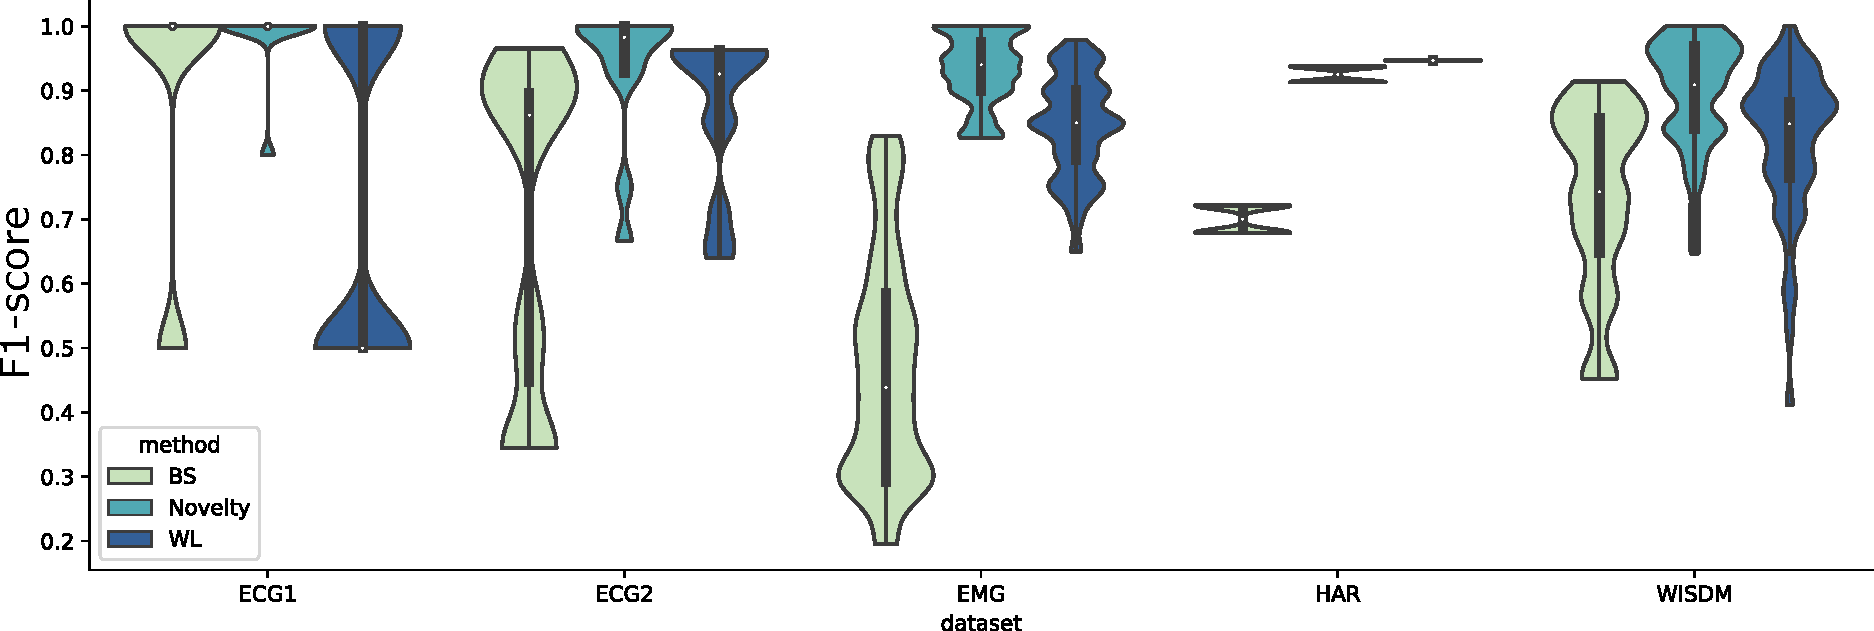
\includegraphics[width=\textwidth]{SSM_F1_scores_distribution.pdf}
\caption{F1-scores distribution for each method in each dataset. The X-axis indicates the dataset, the Y-axis the F1-scores. The labels of the methods are indicated on the bottom left.}
\label{fig:f1_scores}
\end{figure}

The Figure presents information that corroborates the summary presented in the results section, where the F1-score is typically better for the proposed method, indicating that it is more robust than $WL$ and $BS$ methods for the segmentation task in these datasets.

\begin{table}
    \caption{Parameter configuration and experimental results of each signal in Dataset 3 (see Section \ref{dat:dataset3}). $W_{size}$: window size; $K$: kernel size in ratio of the window size; $O$: overlap ratio of the window size. $T$: amplitude threshold ratio for the event detection; Novelty: our proposed method with the novelty function; WL: window-based segmentation; BS: binary segmentation. The tolerance used to calculate the F1-score ($F1$) equals the window size for novelty function computation.}
    \centering
    \begin{tabular}{ccccccccc}
    \toprule
    & \multicolumn{5}{c}{Novelty} & \multicolumn{2}{c}{WL} & BS\\
    \midrule
    Signal &     $W_{size}$ &     $K$ &     $O$ &   $T$    &     $F1$ & $W_{size}$ & $F1$ & $F1$\\
    \cmidrule(lr){2-6} \cmidrule(lr){7-8} \cmidrule(lr){9-9}
    1 & 1500 & 1.5 & 0.90 & 0.01 & 0.91 & 1500 & 0.95 & 0.68 \\
    2 & 1500 & 1.5 & 0.90 & 0.01 & 0.94 & 1500 & 0.95 & 0.72 \\
    \bottomrule
    \end{tabular}
    \label{tab:params_results_1}
\end{table}


\begin{table}[h]
    \caption{Parameter configuration and experimental results of each signal in Dataset 6 (see Section \ref{dat:dataset6}). $W_{size}$: window size; $K$: kernel size in ratio of the window size; $O$: overlap ratio of the window size. $T$: amplitude threshold for event detection; Novelty: our proposed method with the novelty function; WL: window-based segmentation; BS: binary segmentation. The tolerance used to calculate the F1-score ($F1$) equals the window size for novelty function computation.}
    \centering
    \begin{tabular}{ccccccccc}
    \toprule
     & \multicolumn{5}{c}{Novelty} & \multicolumn{2}{c}{WL} & BS\\
    \midrule
    Signal &     $W_{size}$ &     $K()$ &     $O()$ &  $T()$    &     $F1$ & $W_{size}$ & $F1$ & $F1$\\
    \cmidrule(lr){2-6} \cmidrule(lr){7-8} \cmidrule(lr){9-9}\\
    1 & 2000 & 0.62 & 0.95 & 0.19 & 0.90 & 2000 & 0.72 & 0.29 \\ 
    2 & 2000 & 1.25 & 0.95 & 0.28 & 0.86 & 1500 & 0.75 & 0.39 \\ 
    3 & 1500 & 1.27 & 0.95 & 0.10 & 1.00 & 2000 & 0.95 & 0.78 \\ 
    4 & 1500 & 0.63 & 0.95 & 0.14 & 1.00 & 2000 & 0.89 & 0.49 \\ 
    5 & 2000 & 1.25 & 0.95 & 0.28 & 0.92 & 1500 & 0.85 & 0.20 \\ 
    6 & 1500 & 0.63 & 0.95 & 0.28 & 0.88 & 1500 & 0.74 & 0.29 \\ 
    7 & 2000 & 1.25 & 0.95 & 0.19 & 0.95 & 2000 & 0.95 & 0.49 \\ 
    8 & 1500 & 1.27 & 0.95 & 0.10 & 0.93 & 2000 & 0.85 & 0.63 \\ 
    9 & 2000 & 0.62 & 0.95 & 0.28 & 1.00 & 2000 & 0.95 & 0.44 \\ 
    10 & 2000 & 1.25 & 0.95 & 0.28 & 0.97 & 1500 & 0.90 & 0.54 \\ 
    11 & 1000 & 1.25 & 0.95 & 0.10 & 1.00 & 2000 & 0.96 & 0.82 \\ 
    12 & 2000 & 1.25 & 0.95 & 0.14 & 0.83 & 2000 & 0.85 & 0.34 \\ 
    13 & 1000 & 0.62 & 0.95 & 0.37 & 1.00 & 2000 & 0.75 & 0.78 \\ 
    14 & 1000 & 1.25 & 0.95 & 0.32 & 0.95 & 1500 & 0.65 & 0.29 \\ 
    15 & 2000 & 0.62 & 0.95 & 0.14 & 0.93 & 1500 & 0.85 & 0.54 \\ 
    16 & 2000 & 0.62 & 0.95 & 0.28 & 0.90 & 2000 & 0.81 & 0.39 \\ 
    17 & 1500 & 2.53 & 0.95 & 0.10 & 0.98 & 2000 & 0.83 & 0.29 \\ 
    18 & 2000 & 0.62 & 0.95 & 0.50 & 0.97 & 1500 & 0.90 & 0.49 \\ 
    19 & 2000 & 0.62 & 0.95 & 0.23 & 0.93 & 1500 & 0.75 & 0.44 \\ 
    20 & 1500 & 0.63 & 0.95 & 0.10 & 0.95 & 2000 & 0.95 & 0.59 \\ 
    21 & 2000 & 1.25 & 0.95 & 0.19 & 0.95 & 2000 & 0.95 & 0.44 \\ 
    22 & 2000 & 1.25 & 0.95 & 0.19 & 0.84 & 2000 & 0.90 & 0.29 \\ 
    23 & 1500 & 1.27 & 0.95 & 0.28 & 0.90 & 1500 & 0.85 & 0.54 \\ 
    24 & 2000 & 0.62 & 0.95 & 0.19 & 0.86 & 2000 & 0.76 & 0.39 \\ 
    25 & 1500 & 1.27 & 0.95 & 0.37 & 0.95 & 2000 & 0.85 & 0.68 \\ 
    26 & 1500 & 0.63 & 0.95 & 0.19 & 0.98 & 2000 & 0.90 & 0.54 \\ 
    27 & 1500 & 1.27 & 0.95 & 0.19 & 0.83 & 1500 & 0.75 & 0.59 \\ 
    28 & 1500 & 1.27 & 0.95 & 0.37 & 0.90 & 1500 & 0.80 & 0.29 \\ 
    29 & 1500 & 1.27 & 0.95 & 0.23 & 1.00 & 2000 & 0.76 & 0.34 \\ 
    30 & 2000 & 2.5 & 0.95 & 0.10 & 0.92 & 2000 & 0.83 & 0.20 \\ 
    31 & 1000 & 1.25 & 0.95 & 0.19 & 1.00 & 1500 & 0.90 & 0.73 \\ 
    32 & 1500 & 1.27 & 0.95 & 0.41 & 0.89 & 2000 & 0.77 & 0.29 \\ 
    33 & 2000 & 0.62 & 0.95 & 0.23 & 0.83 & 1500 & 0.80 & 0.63 \\ 
    34 & 2000 & 0.62 & 0.95 & 0.28 & 0.93 & 1000 & 0.70 & 0.34 \\ 
    35 & 1500 & 0.63 & 0.95 & 0.14 & 0.95 & 2000 & 0.84 & 0.83 \\ 
    36 & 1000 & 2.5 & 0.95 & 0.14 & 1.00 & 1500 & 0.80 & 0.29 \\ 
    \bottomrule
    \end{tabular}
    \label{tab:params_results_4}
\end{table}

\begin{table}[h]
    \caption{Parameter configuration and experimental results of each signal in Dataset 7 (see Section \ref{dat:dataset7}). $W_{size}$: window size; $K$: kernel size in ratio of the window size; $O$: overlap ratio of the window size. $T$: amplitude threshold for event detection; Novelty: our proposed method with the novelty function; WL: window-based segmentation; BS: binary segmentation. The tolerance used to calculate the F1-score ($F1$) equals the window size for novelty function computation.}
    \centering
    \begin{tabular}{ccccccccc}
    \toprule
    & \multicolumn{5}{c}{Novelty} & \multicolumn{2}{c}{WL} & BS\\
    \midrule
    Signal &     $W_{size}$ &     $K$ &     $O$ &   $T$    &     $F1$ & $W_{size}$ & $F1$ & $F1$\\
    \cmidrule(lr){2-6} \cmidrule(lr){7-8} \cmidrule(lr){9-9}\\
            1 & 1500 & 6.33 & 0.95 & 0.14 & 1.00 & 5000 & 0.93 & 0.97 \\ 
        2 & 5000 & 6.25 & 0.95 & 0.19 & 0.97 & 5000 & 0.79 & 0.97 \\ 
        3 & 5000 & 12.5 & 0.95 & 0.23 & 0.80 & 5000 & 0.57 & 0.83 \\ 
        4 & 3500 & 12.57 & 0.95 & 0.23 & 0.50 & 3500 & 0.21 & 0.48 \\ 
        5 & 5000 & 12.5 & 0.95 & 0.23 & 0.42 & 3500 & 0.14 & 0.34 \\ 
        6 & 1500 & 6.33 & 0.95 & 0.10 & 1.00 & 2500 & 0.93 & 0.90 \\ 
        7 & 2500 & 2.52 & 0.95 & 0.28 & 1.00 & 3500 & 0.86 & 0.90 \\ 
        8 & 2500 & 6.3 & 0.95 & 0.19 & 1.00 & 3500 & 0.64 & 0.90 \\ 
        9 & 2500 & 6.3 & 0.95 & 0.28 & 0.87 & 2500 & 0.29 & 0.55 \\ 
        10 & 5000 & 6.25 & 0.95 & 0.28 & 0.63 & 5000 & 0.21 & 0.34 \\ 
        11 & 5000 & 6.25 & 0.95 & 0.37 & 0.36 & 2500 & 0.07 & 0.34 \\ 
        12 & 2500 & 2.52 & 0.95 & 0.19 & 1.00 & 3500 & 0.93 & 0.90 \\ 
    \bottomrule
    \end{tabular}
    \label{tab:params_results_3}
\end{table}

\begin{table}[h]
    \caption{Parameter configuration and experimental results of each signal in Dataset 8 (see Section \ref{dat:dataset8}). $W_{size}$: window size; $K$: kernel size in ratio of the window size; $O$: overlap ratio of the window size. $T$: amplitude threshold for event detection; Novelty: our proposed method with the novelty function; WL: window-based segmentation; BS: binary segmentation. The tolerance used to calculate the F1-score ($F1$) equals the window size for novelty function computation.}
    \centering
    \begin{tabular}{ccccccccc}
    \toprule
    & \multicolumn{5}{c}{Novelty} & \multicolumn{2}{c}{WL} & BS\\
    \midrule
    Signal &     $W_{size}$ &     $K$ &     $O$ &   $T$    &     $F1$ & $W_{size}$ & $F1$ & $F1$\\
\cmidrule(lr){2-6} \cmidrule(lr){7-8} \cmidrule(lr){9-9}\\

        1 & 400 & 3.74 & 0.95 & 0.55 & 1.00 & 2000 & 0.67 & 0.40 \\ 
        2 & 400 & 2.49 & 0.95 & 0.68 & 0.80 & 400 & 1.00 & 0.40 \\ 
        3 & 150 & 4 & 0.95 & 0.82 & 0.80 & 150 & 0.00 & 0.00 \\ 
        4 & 150 & 2.66 & 0.95 & 0.32 & 1.00 & 2000 & 0.67 & 0.80 \\ 
        5 & 300 & 2.66 & 0.95 & 0.32 & 1.00 & 300 & 1.00 & 0.80 \\ 
        6 & 300 & 2.66 & 0.95 & 0.59 & 1.00 & 1000 & 0.67 & 0.80 \\ 
        7 & 150 & 2.66 & 0.95 & 0.64 & 1.00 & 2000 & 0.67 & 0.80 \\ 
        8 & 150 & 2.66 & 0.95 & 0.28 & 1.00 & 150 & 0.50 & 0.40 \\ 
        9 & 150 & 2.66 & 0.95 & 0.55 & 1.00 & 150 & 0.00 & 0.80 \\ 
    \bottomrule
    \end{tabular}
    \label{tab:params_results_4}
\end{table}
%
%\begin{longtable}[c]{ccccccccc}
%\caption{Parameter configuration and experimental results of each signal in Dataset 13 (see Section \ref{dat:dataset13}). $W_{size}$: window size; $K$: kernel size in ratio of the window size; $O$: overlap ratio of the window size. $T$: amplitude threshold for event detection; Novelty: our proposed method with the novelty function; WL: window-based segmentation; BS: binary segmentation. The tolerance used to calculate the F1-score ($F1$) equals the window size for novelty function computation.}
%\label{tab:params_results_7}\\
%\toprule
%    & \multicolumn{5}{c}{Novelty} & \multicolumn{2}{c}{WL} & BS\\
%    \midrule
%    Signal &     $W_{size}$ &     $K$ &     $O$ &   $T$    &     $F1$ & $W_{size}$ & $F1$ & $F1$\\
%    \cmidrule(lr){2-6} \cmidrule(lr){7-8} \cmidrule(lr){9-9}\\
%
%\endfirsthead
%
%
%\multicolumn{9}{c}{Continuation of Table \ref{tab:params_results_7}}\\
%
%    & \multicolumn{5}{c}{Novelty} & \multicolumn{2}{c}{WL} & BS\\
%    \midrule
%    Signal &     $W_{size}$ &     $K$ &     $T$ &   $O$    &     $F1$ & $W_{size}$ & $F1$ & $F1$\\
%    \cmidrule(lr){2-6} \cmidrule(lr){7-8} \cmidrule(lr){9-9}\\
% \endhead
% \endfoot
% \multicolumn{9}{c}{End of Table}\\
% \endlastfoot
%
%0   &  2000 &  2.49 &  0.36 &  0.95 &  0.93 &  2500 &  0.88 &  0.62 \\
%1   &  2500 &  1.25 &  0.01 &  0.95 &  0.88 &  2500 &  0.71 &  0.75 \\
%2   &  2000 &  1.25 &  0.16 &  0.95 &  0.89 &  2500 &  0.86 &  0.75 \\
%3   &  2500 &  1.26 &  0.41 &  0.95 &  0.80 &  2500 &  0.88 &  0.75 \\
%4   &  2500 &  1.25 &  0.31 &  0.95 &  0.88 &  2000 &  0.75 &  0.75 \\
%5   &  2000 &  1.25 &  0.31 &  0.95 &  0.88 &  2000 &  0.86 &  0.71 \\
%6   &  2500 &  0.75 &  0.50 &  0.95 &  1.00 &  2500 &  0.86 &  0.88 \\
%7   &  2000 &  1.25 &  0.31 &  0.95 &  0.94 &  2000 &  0.93 &  0.71 \\
%8   &  2000 &  1.87 &  0.01 &  0.95 &  0.93 &  2000 &  0.71 &  0.75 \\
%9   &  2500 &  1.25 &  0.01 &  0.95 &  0.88 &  2000 &  0.80 &  0.62 \\
%10  &  2500 &  1.26 &  0.01 &  0.95 &  0.93 &  2000 &  0.86 &  0.71 \\
%11  &  2000 &  1.25 &  0.50 &  0.95 &  0.88 &  2000 &  0.88 &  0.62 \\
%12  &  2500 &  0.75 &  0.21 &  0.95 &  0.93 &  2000 &  0.86 &  0.82 \\
%13  &  1000 &  1.87 &  0.41 &  0.95 &  0.89 &  2000 &  0.77 &  0.62 \\
%14  &  2500 &  0.38 &  0.41 &  0.95 &  0.93 &  2000 &  0.75 &  0.71 \\
%15  &  2000 &  1.25 &  0.21 &  0.95 &  0.86 &  2000 &  0.88 &  0.71 \\
%16  &  2500 &  0.75 &  0.46 &  0.95 &  0.93 &  2000 &  0.86 &  0.75 \\
%17  &  2000 &  1.25 &  0.21 &  0.95 &  0.93 &  2500 &  0.86 &  0.62 \\
%18  &  2500 &  0.38 &  0.36 &  0.95 &  1.00 &  2500 &  0.86 &  0.59 \\
%19  &  2500 &  1.26 &  0.16 &  0.95 &  0.86 &  2000 &  0.88 &  0.62 \\
%20  &  2500 &  0.50 &  0.41 &  0.95 &  0.89 &  2500 &  0.77 &  0.82 \\
%21  &  2000 &  0.62 &  0.36 &  0.95 &  0.84 &  2000 &  0.80 &  0.67 \\
%22  &  2000 &  1.25 &  0.26 &  0.95 &  0.88 &  2000 &  0.71 &  0.71 \\
%23  &  2000 &  1.25 &  0.41 &  0.95 &  0.93 &  2000 &  0.86 &  0.71 \\
%24  &  2500 &  0.63 &  0.46 &  0.95 &  0.93 &  2000 &  0.80 &  0.75 \\
%25  &  2000 &  1.25 &  0.21 &  0.95 &  0.86 &  2500 &  0.77 &  0.71 \\
%26  &  2000 &  1.25 &  0.21 &  0.95 &  0.93 &  2500 &  0.77 &  0.75 \\
%27  &  2000 &  0.50 &  0.46 &  0.95 &  0.88 &  2000 &  0.57 &  0.88 \\
%28  &  2500 &  0.75 &  0.16 &  0.95 &  0.88 &  2500 &  0.77 &  0.82 \\
%29  &  2000 &  0.75 &  0.31 &  0.95 &  0.94 &  2000 &  0.71 &  0.71 \\
%30  &  2000 &  0.50 &  0.46 &  0.95 &  0.88 &  2000 &  0.77 &  0.88 \\
%31  &  2000 &  1.25 &  0.11 &  0.95 &  0.86 &  2500 &  0.62 &  0.59 \\
%32  &  2000 &  1.25 &  0.16 &  0.95 &  0.89 &  2000 &  0.86 &  0.88 \\
%33  &  2000 &  0.37 &  0.36 &  0.95 &  0.86 &  2000 &  0.77 &  0.82 \\
%34  &  2000 &  0.75 &  0.36 &  0.95 &  0.88 &  2000 &  0.88 &  0.75 \\
%35  &  1000 &  1.25 &  0.36 &  0.95 &  0.82 &  2500 &  0.67 &  0.62 \\
%36  &  2500 &  0.63 &  0.11 &  0.95 &  0.80 &  2500 &  0.77 &  0.82 \\
%37  &  2000 &  0.37 &  0.41 &  0.95 &  0.80 &  2000 &  0.67 &  0.82 \\
%38  &  1000 &  1.87 &  0.41 &  0.95 &  0.94 &  2000 &  0.53 &  0.62 \\
%39  &  2500 &  1.26 &  0.01 &  0.95 &  0.80 &  2500 &  0.67 &  0.59 \\
%40  &  2000 &  0.37 &  0.36 &  0.95 &  0.93 &  2000 &  0.80 &  0.62 \\
%41  &  2000 &  0.62 &  0.36 &  0.95 &  0.80 &  2000 &  0.71 &  0.59 \\
%42  &  1000 &  1.25 &  0.46 &  0.95 &  0.89 &  2000 &  0.77 &  0.62 \\
%43  &  2500 &  0.75 &  0.01 &  0.95 &  0.88 &  2500 &  0.67 &  0.71 \\
%44  &  2000 &  0.50 &  0.46 &  0.95 &  1.00 &  2500 &  0.67 &  0.88 \\
%45  &  2000 &  0.75 &  0.31 &  0.95 &  0.80 &  2000 &  0.67 &  0.59 \\
%46  &  2500 &  0.50 &  0.21 &  0.95 &  0.93 &  2000 &  0.77 &  0.88 \\
%47  &  2000 &  0.62 &  0.36 &  0.95 &  0.88 &  2000 &  0.77 &  0.56 \\
%48  &  2500 &  0.25 &  0.36 &  0.95 &  0.93 &  1000 &  0.75 &  0.88 \\
%49  &  2500 &  1.25 &  0.01 &  0.95 &  0.92 &  1000 &  0.57 &  0.67 \\
%50  &  2000 &  1.25 &  0.16 &  0.95 &  0.92 &  2500 &  0.67 &  0.71 \\
%51  &  1000 &  1.87 &  0.26 &  0.95 &  0.80 &  2500 &  0.67 &  0.62 \\
%52  &  2500 &  0.38 &  0.26 &  0.95 &  0.88 &  2000 &  0.80 &  0.59 \\
%53  &  2000 &  0.75 &  0.31 &  0.95 &  0.88 &  2000 &  0.80 &  0.88 \\
%54  &  2500 &  0.38 &  0.31 &  0.95 &  1.00 &  2000 &  0.86 &  0.67 \\
%55  &  2500 &  1.26 &  0.01 &  0.95 &  0.86 &  2000 &  0.80 &  0.62 \\
%56  &  2000 &  0.75 &  0.16 &  0.95 &  0.88 &  2000 &  0.80 &  0.62 \\
%57  &  2500 &  0.75 &  0.31 &  0.95 &  0.57 &  2500 &  0.71 &  0.50 \\
%58  &  2000 &  1.87 &  0.06 &  0.95 &  0.93 &  2000 &  0.75 &  0.71 \\
%59  &  2000 &  0.50 &  0.26 &  0.95 &  0.78 &  2000 &  0.67 &  0.71 \\
%60  &  2000 &  0.37 &  0.31 &  0.95 &  0.88 &  2500 &  0.77 &  0.62 \\
%61  &  2000 &  1.25 &  0.26 &  0.95 &  0.86 &  2000 &  0.88 &  0.62 \\
%62  &  2000 &  1.25 &  0.16 &  0.95 &  0.86 &  2500 &  0.77 &  0.75 \\
%63  &  2000 &  1.25 &  0.01 &  0.95 &  0.86 &  2500 &  0.77 &  0.62 \\
%64  &  2500 &  0.38 &  0.26 &  0.95 &  0.94 &  2500 &  0.77 &  0.71 \\
%65  &  2000 &  1.87 &  0.01 &  0.95 &  0.80 &  2000 &  0.80 &  0.62 \\
%66  &  2500 &  0.38 &  0.31 &  0.95 &  1.00 &  2000 &  0.88 &  0.88 \\
%67  &  2500 &  1.25 &  0.01 &  0.95 &  0.86 &  2000 &  0.77 &  0.62 \\
%68  &  2500 &  0.38 &  0.36 &  0.95 &  0.93 &  2000 &  0.88 &  0.75 \\
%69  &  2000 &  1.25 &  0.26 &  0.95 &  0.86 &  2000 &  0.80 &  0.75 \\
%70  &  2500 &  0.63 &  0.16 &  0.95 &  1.00 &  2000 &  0.86 &  0.62 \\
%71  &  2500 &  1.26 &  0.01 &  0.95 &  0.86 &  2000 &  0.80 &  0.67 \\
%72  &  2500 &  0.75 &  0.16 &  0.95 &  0.93 &  2000 &  0.88 &  0.88 \\
%73  &  2000 &  1.25 &  0.11 &  0.95 &  0.86 &  2000 &  0.88 &  0.62 \\
%74  &  2000 &  0.37 &  0.36 &  0.95 &  0.88 &  2500 &  0.77 &  0.75 \\
%75  &  2000 &  0.62 &  0.26 &  0.95 &  0.89 &  2500 &  0.77 &  0.71 \\
%76  &  2000 &  0.62 &  0.16 &  0.95 &  1.00 &  2500 &  0.77 &  0.62 \\
%77  &  2000 &  0.62 &  0.26 &  0.95 &  0.93 &  2000 &  0.71 &  0.75 \\
%78  &  2000 &  0.62 &  0.26 &  0.95 &  0.94 &  2000 &  0.77 &  0.62 \\
%79  &  2000 &  0.50 &  0.36 &  0.95 &  0.93 &  2000 &  0.80 &  0.62 \\
%80  &  2500 &  0.50 &  0.16 &  0.95 &  0.94 &  2000 &  0.86 &  0.75 \\
%81  &  2500 &  0.50 &  0.31 &  0.95 &  0.88 &  2000 &  0.77 &  0.59 \\
%82  &  2500 &  0.25 &  0.26 &  0.95 &  0.93 &  2000 &  0.86 &  0.59 \\
%83  &  2000 &  1.25 &  0.26 &  0.95 &  0.86 &  2500 &  0.77 &  0.59 \\
%84  &  2500 &  0.38 &  0.26 &  0.95 &  0.93 &  2000 &  0.71 &  0.71 \\
%85  &  2000 &  1.25 &  0.11 &  0.95 &  0.86 &  2000 &  0.80 &  0.75 \\
%86  &  2000 &  0.75 &  0.16 &  0.95 &  0.86 &  2000 &  0.71 &  0.62 \\
%87  &  2000 &  1.25 &  0.16 &  0.95 &  0.86 &  2000 &  0.77 &  0.62 \\
%88  &  2500 &  0.38 &  0.31 &  0.95 &  0.94 &  2000 &  0.80 &  0.75 \\
%89  &  2000 &  0.62 &  0.31 &  0.95 &  0.88 &  2000 &  0.86 &  0.62 \\
%90  &  2500 &  0.50 &  0.36 &  0.95 &  0.89 &  2000 &  0.86 &  0.78 \\
%91  &  2500 &  1.25 &  0.11 &  0.95 &  0.80 &  2500 &  0.77 &  0.56 \\
%92  &  2500 &  0.63 &  0.11 &  0.95 &  0.93 &  2000 &  0.86 &  0.56 \\
%93  &  2000 &  0.62 &  0.21 &  0.95 &  0.88 &  2000 &  0.71 &  0.59 \\
%94  &  2000 &  0.50 &  0.46 &  0.95 &  0.93 &  2000 &  0.71 &  0.67 \\
%95  &  2000 &  0.62 &  0.41 &  0.95 &  0.89 &  2000 &  0.77 &  0.62 \\
%96  &  2500 &  0.50 &  0.21 &  0.95 &  0.93 &  2000 &  0.77 &  0.88 \\
%97  &  2000 &  0.75 &  0.36 &  0.95 &  0.93 &  2000 &  0.86 &  0.62 \\
%98  &  2000 &  0.62 &  0.21 &  0.95 &  0.94 &  2000 &  0.86 &  0.71 \\
%99  &  2000 &  1.25 &  0.16 &  0.95 &  0.86 &  2000 &  0.77 &  0.59 \\
%100 &  2000 &  0.50 &  0.46 &  0.95 &  0.93 &  2000 &  0.86 &  0.75 \\
%101 &  2000 &  1.25 &  0.16 &  0.95 &  0.86 &  2000 &  0.86 &  0.62 \\
%102 &  2500 &  1.26 &  0.36 &  0.95 &  0.93 &  2500 &  0.88 &  0.75 \\
%103 &  2000 &  1.25 &  0.31 &  0.95 &  0.84 &  2000 &  0.62 &  0.38 \\
%104 &  2000 &  0.62 &  0.36 &  0.95 &  0.94 &  2000 &  0.88 &  0.75 \\
%105 &  2000 &  0.62 &  0.41 &  0.95 &  0.88 &  1000 &  0.59 &  0.75 \\
%106 &  2000 &  1.25 &  0.26 &  0.95 &  0.93 &  2000 &  0.88 &  0.62 \\
%107 &  2500 &  0.75 &  0.21 &  0.95 &  1.00 &  2500 &  0.77 &  1.00 \\
%108 &  1000 &  2.50 &  0.16 &  0.95 &  0.93 &  2000 &  0.62 &  0.62 \\
%109 &  2000 &  0.25 &  0.36 &  0.95 &  0.93 &  2000 &  0.80 &  0.62 \\
%110 &  2500 &  0.13 &  0.26 &  0.95 &  1.00 &  2000 &  0.88 &  0.75 \\
%111 &  2000 &  1.25 &  0.01 &  0.95 &  0.88 &  2000 &  0.88 &  0.59 \\
%112 &  2000 &  0.62 &  0.46 &  0.95 &  0.88 &  2000 &  0.86 &  0.47 \\
%113 &  2000 &  0.50 &  0.41 &  0.95 &  0.89 &  2000 &  0.77 &  0.62 \\
%114 &  2000 &  0.62 &  0.16 &  0.95 &  0.94 &  2000 &  0.86 &  0.75 \\
%115 &  1000 &  2.50 &  0.26 &  0.95 &  0.88 &  2000 &  0.67 &  0.88 \\
%116 &  2000 &  1.25 &  0.01 &  0.95 &  0.88 &  2000 &  0.80 &  0.75 \\
%117 &  1000 &  1.87 &  0.26 &  0.95 &  0.88 &  2500 &  0.57 &  0.50 \\
%118 &  2000 &  0.62 &  0.16 &  0.95 &  0.89 &  2000 &  0.71 &  0.75 \\
%119 &  2500 &  0.75 &  0.21 &  0.95 &  0.88 &  2500 &  0.77 &  0.62 \\
%120 &  2000 &  1.25 &  0.26 &  0.95 &  1.00 &  2000 &  0.75 &  0.62 \\
%121 &  2500 &  0.63 &  0.16 &  0.95 &  0.94 &  2000 &  0.75 &  0.62 \\
%122 &  2500 &  0.63 &  0.16 &  0.95 &  0.94 &  2000 &  0.88 &  0.59 \\
%123 &  2500 &  1.26 &  0.01 &  0.95 &  0.86 &  2000 &  0.82 &  0.56 \\
%124 &  2500 &  0.25 &  0.31 &  0.95 &  1.00 &  2000 &  0.86 &  0.88 \\
%125 &  2000 &  1.25 &  0.16 &  0.95 &  0.88 &  2000 &  0.88 &  0.75 \\
%126 &  2000 &  1.25 &  0.26 &  0.95 &  0.93 &  2000 &  0.86 &  0.75 \\
%127 &  2000 &  1.25 &  0.26 &  0.95 &  0.93 &  2000 &  0.80 &  0.62 \\
%128 &  2000 &  0.75 &  0.21 &  0.95 &  0.94 &  2000 &  0.88 &  0.75 \\
%129 &  2500 &  0.75 &  0.01 &  0.95 &  0.89 &  2000 &  0.88 &  0.75 \\
%130 &  2500 &  1.26 &  0.01 &  0.95 &  0.86 &  2500 &  0.86 &  0.75 \\
%131 &  2000 &  1.87 &  0.01 &  0.95 &  0.80 &  2500 &  0.86 &  0.50 \\
%132 &  2000 &  1.87 &  0.01 &  0.95 &  0.86 &  2000 &  0.88 &  0.62 \\
%133 &  2500 &  0.38 &  0.31 &  0.95 &  0.88 &  2000 &  0.71 &  0.75 \\
%134 &  2500 &  0.63 &  0.26 &  0.95 &  0.88 &  2000 &  0.77 &  0.59 \\
%135 &  2500 &  0.25 &  0.26 &  0.95 &  0.93 &  2000 &  0.77 &  0.88 \\
%136 &  2500 &  0.50 &  0.21 &  0.95 &  0.89 &  2000 &  0.67 &  0.59 \\
%137 &  2000 &  0.62 &  0.31 &  0.95 &  0.82 &  2000 &  0.86 &  0.62 \\
%138 &  2500 &  0.63 &  0.16 &  0.95 &  0.94 &  2000 &  0.93 &  0.62 \\
%139 &  2500 &  0.63 &  0.26 &  0.95 &  0.94 &  2000 &  0.82 &  0.59 \\
%140 &  2500 &  0.75 &  0.41 &  0.95 &  0.94 &  2000 &  0.94 &  0.82 \\
%141 &  2000 &  1.25 &  0.31 &  0.95 &  0.86 &  2000 &  0.80 &  0.62 \\
%142 &  2500 &  0.50 &  0.16 &  0.95 &  0.89 &  2000 &  0.80 &  0.59 \\
%143 &  1000 &  2.50 &  0.26 &  0.95 &  0.88 &  2000 &  0.57 &  0.50 \\
%144 &  2500 &  0.63 &  0.16 &  0.95 &  0.94 &  2000 &  0.67 &  0.75 \\
%145 &  2500 &  0.63 &  0.11 &  0.95 &  0.84 &  2000 &  0.93 &  0.62 \\
%146 &  2500 &  0.75 &  0.21 &  0.95 &  0.80 &  2000 &  0.75 &  0.62 \\
%147 &  2500 &  2.51 &  0.01 &  0.95 &  0.93 &  2000 &  0.88 &  0.62 \\
%148 &  2500 &  1.88 &  0.01 &  0.95 &  0.93 &  2000 &  0.75 &  0.62 \\
%149 &  2000 &  0.62 &  0.46 &  0.95 &  0.88 &  2000 &  0.88 &  0.62 \\
%150 &  2500 &  0.13 &  0.31 &  0.95 &  0.86 &  2500 &  0.88 &  0.62 \\
%151 &  2000 &  0.50 &  0.46 &  0.95 &  0.88 &  2000 &  0.88 &  0.62 \\
%152 &  2500 &  1.26 &  0.46 &  0.95 &  0.93 &  2500 &  0.93 &  0.62 \\
%153 &  2000 &  1.87 &  0.11 &  0.95 &  0.88 &  2000 &  0.67 &  0.75 \\
%154 &  2500 &  1.88 &  0.01 &  0.95 &  0.93 &  2000 &  0.75 &  0.50 \\
%155 &  2500 &  0.75 &  0.01 &  0.95 &  0.84 &  2500 &  0.86 &  0.62 \\
%156 &  2500 &  1.25 &  0.01 &  0.95 &  0.94 &  2500 &  0.77 &  0.62 \\
%157 &  2500 &  1.88 &  0.01 &  0.95 &  0.86 &  2500 &  0.93 &  0.62 \\
%158 &  2500 &  0.63 &  0.26 &  0.95 &  0.84 &  2000 &  0.88 &  0.62 \\
%159 &  2500 &  1.88 &  0.01 &  0.95 &  0.80 &  2500 &  0.67 &  0.62 \\
%160 &  2000 &  1.87 &  0.01 &  0.95 &  0.88 &  2500 &  0.93 &  0.62 \\
%161 &  2500 &  2.51 &  0.01 &  0.95 &  0.86 &  2500 &  0.80 &  0.62 \\
%162 &  2000 &  1.25 &  0.16 &  0.95 &  0.94 &  2000 &  0.88 &  0.88 \\
%163 &  2000 &  0.62 &  0.46 &  0.95 &  0.89 &  2000 &  1.00 &  0.75 \\
%164 &  2000 &  1.25 &  0.21 &  0.95 &  0.89 &  2500 &  0.93 &  0.62 \\
%165 &  2500 &  0.50 &  0.16 &  0.95 &  0.80 &  2500 &  0.80 &  0.62 \\
%166 &  2500 &  1.26 &  0.41 &  0.95 &  0.93 &  2500 &  0.86 &  0.62 \\
%167 &  2500 &  0.75 &  0.01 &  0.95 &  0.82 &  2500 &  0.93 &  0.62 \\
%168 &  2000 &  1.87 &  0.01 &  0.95 &  0.88 &  2000 &  0.88 &  0.62 \\
%169 &  2500 &  1.88 &  0.01 &  0.95 &  0.86 &  2000 &  0.80 &  0.59 \\
%170 &  2500 &  1.26 &  0.36 &  0.95 &  0.86 &  2000 &  0.88 &  0.59 \\
%171 &  2000 &  1.25 &  0.36 &  0.95 &  0.82 &  2000 &  0.93 &  0.62 \\
%172 &  2500 &  1.26 &  0.01 &  0.95 &  0.80 &  2500 &  0.93 &  0.75 \\
%173 &  2000 &  1.25 &  0.41 &  0.95 &  0.88 &  2000 &  0.88 &  0.75 \\
%174 &  2000 &  1.25 &  0.11 &  0.95 &  0.82 &  2000 &  0.75 &  0.75 \\
%175 &  2500 &  0.75 &  0.11 &  0.95 &  0.82 &  2500 &  0.86 &  0.62 \\
%176 &  2000 &  1.87 &  0.01 &  0.95 &  0.82 &  2500 &  0.88 &  0.62 \\
%177 &  2000 &  1.87 &  0.01 &  0.95 &  0.74 &  1000 &  0.62 &  0.62 \\
%178 &  2500 &  0.13 &  0.21 &  0.95 &  0.88 &  2500 &  0.93 &  0.75 \\
%179 &  2500 &  0.75 &  0.01 &  0.95 &  0.94 &  2000 &  0.88 &  0.75 \\
%180 &  2500 &  1.26 &  0.01 &  0.95 &  0.88 &  2000 &  0.86 &  0.71 \\
%181 &  2000 &  1.25 &  0.46 &  0.95 &  0.88 &  2500 &  0.80 &  0.62 \\
%182 &  2500 &  1.26 &  0.01 &  0.95 &  1.00 &  2000 &  0.86 &  0.59 \\
%183 &  2500 &  0.63 &  0.55 &  0.95 &  0.86 &  2000 &  0.86 &  0.62 \\
%184 &  2000 &  1.25 &  0.01 &  0.95 &  0.82 &  2500 &  0.93 &  0.75 \\
%185 &  2500 &  0.75 &  0.01 &  0.95 &  0.82 &  2000 &  0.88 &  0.75 \\
%186 &  2000 &  1.25 &  0.11 &  0.95 &  0.82 &  2500 &  0.82 &  0.78 \\
%187 &  2500 &  1.26 &  0.11 &  0.95 &  0.82 &  2000 &  0.88 &  0.67 \\
%188 &  2000 &  1.25 &  0.11 &  0.95 &  0.88 &  2500 &  0.93 &  0.75 \\
%189 &  2000 &  1.25 &  0.41 &  0.95 &  0.82 &  2500 &  0.67 &  0.75 \\
%190 &  2000 &  1.87 &  0.01 &  0.95 &  1.00 &  2000 &  0.88 &  0.75 \\
%191 &  2500 &  1.26 &  0.01 &  0.95 &  0.80 &  2000 &  0.86 &  0.62 \\
%192 &  2500 &  1.25 &  0.31 &  0.95 &  0.82 &  2000 &  0.80 &  0.67 \\
%193 &  2500 &  0.38 &  0.31 &  0.95 &  1.00 &  2000 &  0.80 &  0.82 \\
%194 &  2000 &  1.87 &  0.16 &  0.95 &  0.93 &  2000 &  0.93 &  0.62 \\
%195 &  2500 &  0.75 &  0.41 &  0.95 &  1.00 &  2500 &  0.86 &  0.71 \\
%196 &  2000 &  0.62 &  0.31 &  0.95 &  0.89 &  2500 &  0.71 &  0.62 \\
%197 &  2500 &  1.26 &  0.01 &  0.95 &  0.93 &  2500 &  0.86 &  0.75 \\
%198 &  2000 &  1.25 &  0.31 &  0.95 &  0.88 &  2500 &  0.86 &  0.62 \\
%199 &  2500 &  0.38 &  0.31 &  0.95 &  0.94 &  2000 &  0.88 &  0.75 \\
%200 &  2000 &  1.25 &  0.46 &  0.95 &  0.80 &  2000 &  0.88 &  0.75 \\
%201 &  2500 &  1.25 &  0.01 &  0.95 &  0.93 &  2000 &  0.88 &  0.71 \\
%202 &  2500 &  1.26 &  0.01 &  0.95 &  0.93 &  2000 &  0.75 &  0.75 \\
%203 &  2500 &  0.50 &  0.36 &  0.95 &  0.93 &  2000 &  0.82 &  0.71 \\
%204 &  2000 &  1.25 &  0.26 &  0.95 &  0.84 &  2500 &  0.86 &  0.62 \\
%205 &  2500 &  0.75 &  0.50 &  0.95 &  0.93 &  2000 &  0.88 &  0.78 \\
%206 &  2000 &  1.25 &  0.50 &  0.95 &  0.82 &  2000 &  0.86 &  0.75 \\
%207 &  2500 &  0.50 &  0.41 &  0.95 &  0.93 &  2000 &  0.86 &  0.82 \\
%208 &  2000 &  1.25 &  0.11 &  0.95 &  0.82 &  2500 &  0.86 &  0.62 \\
%209 &  2500 &  0.38 &  0.31 &  0.95 &  1.00 &  2000 &  0.88 &  0.71 \\
%210 &  2500 &  0.63 &  0.31 &  0.95 &  0.88 &  2000 &  0.86 &  0.71 \\
%211 &  2500 &  0.75 &  0.41 &  0.95 &  1.00 &  2000 &  0.88 &  0.71 \\
%212 &  2000 &  0.62 &  0.31 &  0.95 &  0.80 &  2000 &  0.80 &  0.62 \\
%213 &  2500 &  0.75 &  0.41 &  0.95 &  1.00 &  2000 &  0.88 &  0.88 \\
%214 &  2000 &  1.25 &  0.01 &  0.95 &  0.82 &  2000 &  0.86 &  0.62 \\
%215 &  2500 &  0.75 &  0.16 &  0.95 &  1.00 &  2500 &  0.86 &  0.71 \\
%216 &  2000 &  0.50 &  0.36 &  0.95 &  0.89 &  2000 &  0.88 &  0.62 \\
%217 &  2000 &  0.62 &  0.50 &  0.95 &  0.89 &  2000 &  1.00 &  0.75 \\
%218 &  2000 &  1.87 &  0.41 &  0.95 &  0.86 &  2000 &  0.86 &  0.62 \\
%219 &  2500 &  1.25 &  0.16 &  0.95 &  0.93 &  2500 &  0.86 &  0.71 \\
%220 &  2000 &  0.62 &  0.31 &  0.95 &  0.82 &  2000 &  0.88 &  0.62 \\
%221 &  2500 &  0.75 &  0.21 &  0.95 &  1.00 &  2500 &  0.88 &  0.78 \\
%222 &  2000 &  0.50 &  0.50 &  0.95 &  0.82 &  2000 &  0.80 &  0.71 \\
%223 &  2500 &  0.38 &  0.41 &  0.95 &  0.93 &  2500 &  0.86 &  1.00 \\
%224 &  2500 &  1.26 &  0.01 &  0.95 &  0.93 &  2000 &  0.86 &  0.75 \\
%225 &  2000 &  0.75 &  0.36 &  0.95 &  0.94 &  2000 &  0.80 &  0.62 \\
%226 &  2500 &  1.26 &  0.01 &  0.95 &  0.84 &  2500 &  0.86 &  0.62 \\
%227 &  2500 &  0.75 &  0.50 &  0.95 &  1.00 &  2000 &  0.88 &  0.82 \\
%228 &  2500 &  0.25 &  0.21 &  0.95 &  0.82 &  2500 &  0.71 &  0.50 \\
%229 &  2000 &  1.87 &  0.01 &  0.95 &  1.00 &  2000 &  0.86 &  0.75 \\
%230 &  2500 &  1.25 &  0.46 &  0.95 &  0.86 &  2000 &  0.93 &  0.88 \\
%231 &  2500 &  0.63 &  0.36 &  0.95 &  1.00 &  2000 &  0.80 &  0.71 \\
%232 &  2000 &  0.50 &  0.41 &  0.95 &  0.82 &  2000 &  0.71 &  0.62 \\
%233 &  2500 &  0.50 &  0.16 &  0.95 &  1.00 &  2000 &  0.88 &  0.71 \\
%234 &  2000 &  1.25 &  0.21 &  0.95 &  0.82 &  2000 &  0.88 &  0.71 \\
%235 &  2500 &  1.26 &  0.11 &  0.95 &  0.88 &  2000 &  0.88 &  0.50 \\
%236 &  2000 &  1.25 &  0.46 &  0.95 &  0.93 &  2500 &  0.80 &  0.75 \\
%237 &  2500 &  0.63 &  0.21 &  0.95 &  1.00 &  2000 &  0.93 &  0.62 \\
%238 &  2000 &  1.25 &  0.31 &  0.95 &  0.93 &  2500 &  0.86 &  0.71 \\
%239 &  2500 &  0.50 &  0.41 &  0.95 &  0.94 &  2000 &  0.86 &  0.88 \\
%240 &  1000 &  2.50 &  0.55 &  0.95 &  0.94 &  2000 &  0.62 &  0.62 \\
%241 &  2500 &  0.25 &  0.31 &  0.95 &  1.00 &  2000 &  0.88 &  0.59 \\
%242 &  2500 &  0.63 &  0.46 &  0.95 &  0.93 &  2000 &  0.80 &  0.56 \\
%243 &  2500 &  0.25 &  0.21 &  0.95 &  0.89 &  2000 &  0.88 &  0.75 \\
%244 &  2000 &  2.49 &  0.01 &  0.95 &  0.93 &  2500 &  0.80 &  0.62 \\
%245 &  2500 &  0.63 &  0.46 &  0.95 &  1.00 &  2500 &  0.86 &  0.67 \\
%246 &  2000 &  0.25 &  0.36 &  0.95 &  0.89 &  2000 &  0.71 &  0.71 \\
%247 &  2000 &  0.25 &  0.46 &  0.95 &  0.80 &  2500 &  1.00 &  0.75 \\
%248 &  2000 &  0.25 &  0.31 &  0.95 &  0.67 &  2500 &  0.67 &  0.50 \\
%249 &  2000 &  0.50 &  0.36 &  0.95 &  0.89 &  2000 &  0.88 &  0.62 \\
%250 &  2000 &  1.25 &  0.46 &  0.95 &  0.88 &  2000 &  0.80 &  0.62 \\
%251 &  2000 &  0.75 &  0.41 &  0.95 &  0.94 &  2000 &  0.62 &  0.38 \\
%252 &  2500 &  0.25 &  0.31 &  0.95 &  0.89 &  2000 &  0.93 &  0.59 \\
%253 &  2000 &  0.37 &  0.41 &  0.95 &  0.89 &  2000 &  0.93 &  0.75 \\
%254 &  2000 &  1.25 &  0.11 &  0.95 &  0.88 &  2500 &  0.88 &  0.62 \\
%255 &  2500 &  0.63 &  0.46 &  0.95 &  1.00 &  2000 &  0.71 &  0.62 \\
%256 &  2000 &  0.50 &  0.31 &  0.95 &  0.88 &  2000 &  0.93 &  0.62 \\
%257 &  2500 &  0.75 &  0.11 &  0.95 &  1.00 &  2000 &  0.88 &  0.59 \\
%258 &  2000 &  0.50 &  0.26 &  0.95 &  0.89 &  2500 &  0.86 &  0.62 \\
%259 &  2000 &  0.37 &  0.46 &  0.95 &  0.88 &  2000 &  0.93 &  0.88 \\
%260 &  2000 &  0.25 &  0.36 &  0.95 &  0.88 &  2000 &  0.88 &  0.62 \\
%261 &  2500 &  0.63 &  0.50 &  0.95 &  1.00 &  1000 &  0.88 &  0.75 \\
%262 &  2000 &  0.75 &  0.26 &  0.95 &  0.88 &  2000 &  0.88 &  0.75 \\
%263 &  2500 &  0.38 &  0.41 &  0.95 &  1.00 &  2000 &  0.93 &  0.50 \\
%264 &  2500 &  0.63 &  0.01 &  0.95 &  0.88 &  2000 &  0.80 &  0.62 \\
%265 &  2000 &  0.75 &  0.46 &  0.95 &  1.00 &  2000 &  0.86 &  0.50 \\
%266 &  2000 &  1.25 &  0.21 &  0.95 &  0.89 &  2000 &  0.93 &  0.62 \\
%267 &  2000 &  0.50 &  0.46 &  0.95 &  1.00 &  2000 &  0.86 &  0.75 \\
%268 &  2000 &  1.25 &  0.31 &  0.95 &  0.88 &  2000 &  0.93 &  0.62 \\
%269 &  2500 &  0.38 &  0.41 &  0.95 &  1.00 &  2500 &  0.67 &  0.62 \\
%270 &  2000 &  1.25 &  0.21 &  0.95 &  0.88 &  2000 &  0.86 &  0.82 \\
%271 &  2500 &  0.75 &  0.11 &  0.95 &  0.94 &  2000 &  0.86 &  0.75 \\
%272 &  2000 &  0.75 &  0.16 &  0.95 &  0.82 &  2000 &  0.88 &  0.67 \\
%273 &  2500 &  0.50 &  0.21 &  0.95 &  0.89 &  2000 &  0.88 &  0.71 \\
%274 &  2000 &  1.87 &  0.01 &  0.95 &  0.93 &  2000 &  0.86 &  0.62 \\
%275 &  2500 &  0.63 &  0.41 &  0.95 &  1.00 &  2000 &  0.93 &  0.62 \\
%276 &  2000 &  1.87 &  0.41 &  0.95 &  0.86 &  2000 &  0.86 &  0.62 \\
%277 &  2000 &  1.25 &  0.36 &  0.95 &  0.88 &  2500 &  0.67 &  0.50 \\
%278 &  2500 &  0.75 &  0.21 &  0.95 &  0.91 &  2000 &  0.80 &  0.71 \\
%279 &  2000 &  1.87 &  0.01 &  0.95 &  0.86 &  2500 &  0.86 &  0.71 \\
%280 &  2500 &  0.25 &  0.31 &  0.95 &  1.00 &  2000 &  0.86 &  0.62 \\
%281 &  2000 &  0.50 &  0.41 &  0.95 &  0.82 &  2000 &  0.88 &  0.62 \\
%282 &  2500 &  0.38 &  0.36 &  0.95 &  1.00 &  2000 &  0.80 &  0.62 \\
%283 &  2500 &  1.25 &  0.01 &  0.95 &  0.93 &  2000 &  0.88 &  0.62 \\
%284 &  2000 &  0.37 &  0.26 &  0.95 &  0.82 &  1000 &  0.88 &  0.50 \\
%285 &  2500 &  1.25 &  0.01 &  0.95 &  0.91 &  2500 &  0.80 &  0.67 \\
%286 &  2500 &  0.63 &  0.11 &  0.95 &  1.00 &  2000 &  0.82 &  0.63 \\
%287 &  2000 &  1.25 &  0.01 &  0.95 &  0.82 &  2500 &  0.71 &  0.56 \\
%288 &  2000 &  1.87 &  0.01 &  0.95 &  0.88 &  2500 &  0.93 &  0.50 \\
%289 &  2500 &  0.38 &  0.26 &  0.95 &  0.94 &  1000 &  1.00 &  0.62 \\
%290 &  2000 &  0.75 &  0.16 &  0.95 &  0.82 &  2000 &  0.88 &  0.62 \\
%291 &  2000 &  1.25 &  0.31 &  0.95 &  0.88 &  2000 &  0.93 &  0.62 \\
%292 &  2500 &  0.63 &  0.26 &  0.95 &  0.94 &  2000 &  0.80 &  0.75 \\
%293 &  2000 &  1.24 &  0.01 &  0.95 &  0.88 &  2500 &  0.86 &  0.62 \\
%294 &  2500 &  0.38 &  0.16 &  0.95 &  0.94 &  2500 &  0.80 &  0.75 \\
%295 &  2500 &  1.26 &  0.01 &  0.95 &  0.93 &  2500 &  0.86 &  0.62 \\
%296 &  2500 &  0.50 &  0.26 &  0.95 &  0.94 &  2000 &  0.82 &  0.62 \\
%297 &  2000 &  1.25 &  0.01 &  0.95 &  0.82 &  2500 &  0.80 &  0.62 \\
%298 &  2500 &  0.38 &  0.16 &  0.95 &  0.94 &  2000 &  0.88 &  0.62 \\
%299 &  2000 &  1.87 &  0.26 &  0.95 &  0.86 &  2500 &  0.93 &  0.62 \\
%300 &  2000 &  1.25 &  0.01 &  0.95 &  0.88 &  2000 &  0.93 &  0.62 \\
%301 &  2500 &  0.63 &  0.16 &  0.95 &  0.89 &  2500 &  0.86 &  0.71 \\
%302 &  2000 &  0.62 &  0.46 &  0.95 &  0.88 &  2000 &  0.80 &  0.75 \\
%303 &  2500 &  0.75 &  0.11 &  0.95 &  0.89 &  2500 &  0.86 &  0.75 \\
%304 &  2500 &  0.75 &  0.46 &  0.95 &  0.93 &  2000 &  0.86 &  0.75 \\
%305 &  2000 &  1.87 &  0.21 &  0.95 &  0.88 &  2000 &  0.86 &  0.62 \\
%306 &  2000 &  1.25 &  0.31 &  0.95 &  0.88 &  2000 &  0.88 &  0.62 \\
%307 &  2000 &  1.87 &  0.01 &  0.95 &  0.93 &  2000 &  0.93 &  0.62 \\
%308 &  2500 &  0.75 &  0.41 &  0.95 &  1.00 &  2000 &  0.86 &  0.88 \\
%309 &  2000 &  1.25 &  0.36 &  0.95 &  0.93 &  2000 &  0.75 &  0.62 \\
%310 &  1000 &  2.50 &  0.11 &  0.95 &  0.88 &  2500 &  0.86 &  0.50 \\
%311 &  1000 &  1.87 &  0.21 &  0.95 &  0.89 &  2500 &  0.71 &  0.62 \\
%312 &  2000 &  1.25 &  0.26 &  0.95 &  1.00 &  2000 &  0.93 &  0.62 \\
%313 &  2000 &  1.25 &  0.50 &  0.95 &  0.93 &  2000 &  0.93 &  0.62 \\
%314 &  2000 &  1.25 &  0.46 &  0.95 &  0.93 &  2000 &  0.86 &  0.62 \\
%315 &  2500 &  1.26 &  0.21 &  0.95 &  1.00 &  2500 &  0.93 &  0.62 \\
%316 &  2000 &  1.25 &  0.01 &  0.95 &  0.88 &  2000 &  0.86 &  0.62 \\
%317 &  2500 &  0.75 &  0.11 &  0.95 &  0.94 &  2000 &  0.86 &  0.75 \\
%318 &  2500 &  0.75 &  0.11 &  0.95 &  0.94 &  2500 &  0.88 &  0.75 \\
%319 &  1000 &  1.87 &  0.16 &  0.95 &  0.89 &  2000 &  0.86 &  0.62 \\
%320 &  2500 &  0.63 &  0.31 &  0.95 &  0.94 &  2000 &  0.88 &  0.75 \\
%321 &  2000 &  0.75 &  0.36 &  0.95 &  0.89 &  2000 &  0.93 &  0.62 \\
%322 &  2500 &  0.50 &  0.21 &  0.95 &  0.94 &  2000 &  0.88 &  0.62 \\
%323 &  2000 &  0.75 &  0.26 &  0.95 &  0.88 &  2000 &  0.88 &  0.62 \\
%324 &  2500 &  0.75 &  0.01 &  0.95 &  0.89 &  1000 &  0.82 &  0.62 \\
%325 &  2000 &  1.25 &  0.26 &  0.95 &  0.88 &  2000 &  0.93 &  0.62 \\
%326 &  2500 &  0.50 &  0.41 &  0.95 &  1.00 &  1000 &  0.88 &  0.75 \\
%327 &  2500 &  0.75 &  0.11 &  0.95 &  0.88 &  2000 &  0.86 &  0.62 \\
%328 &  2500 &  0.50 &  0.41 &  0.95 &  0.74 &  2000 &  0.75 &  0.75 \\
%329 &  2500 &  1.26 &  0.26 &  0.95 &  0.82 &  2000 &  0.75 &  0.62 \\
%330 &  2500 &  0.50 &  0.26 &  0.95 &  0.94 &  2000 &  0.75 &  0.62 \\
%331 &  2000 &  0.75 &  0.26 &  0.95 &  1.00 &  2000 &  0.93 &  0.62 \\
%332 &  2000 &  0.37 &  0.36 &  0.95 &  0.88 &  2500 &  0.93 &  0.59 \\
%333 &  2500 &  0.63 &  0.41 &  0.95 &  0.89 &  2000 &  0.86 &  0.75 \\
%334 &  2000 &  1.25 &  0.11 &  0.95 &  0.88 &  2500 &  0.93 &  0.59 \\
%335 &  2000 &  0.50 &  0.41 &  0.95 &  0.94 &  2500 &  0.86 &  0.75 \\
%336 &  2500 &  1.88 &  0.01 &  0.95 &  0.86 &  2000 &  0.88 &  0.71 \\
%337 &  2000 &  0.37 &  0.41 &  0.95 &  0.88 &  1000 &  0.88 &  0.62 \\
%338 &  2000 &  1.25 &  0.31 &  0.95 &  0.88 &  2500 &  0.93 &  0.62 \\
%339 &  2500 &  0.63 &  0.31 &  0.95 &  0.88 &  2500 &  0.80 &  0.62 \\
%340 &  2000 &  1.25 &  0.31 &  0.95 &  0.80 &  2500 &  0.86 &  0.62 \\
%341 &  2500 &  1.26 &  0.01 &  0.95 &  0.88 &  2500 &  0.86 &  0.62 \\
%342 &  2500 &  0.38 &  0.36 &  0.95 &  0.80 &  2000 &  0.93 &  0.59 \\
%343 &  2000 &  0.62 &  0.36 &  0.95 &  0.84 &  2500 &  0.80 &  0.62 \\
%344 &  2000 &  0.62 &  0.31 &  0.95 &  0.73 &  2000 &  0.88 &  0.78 \\
%345 &  2000 &  1.25 &  0.01 &  0.95 &  0.82 &  2500 &  0.93 &  0.75 \\
%346 &  2500 &  0.75 &  0.46 &  0.95 &  0.82 &  2000 &  0.93 &  0.71 \\
%347 &  2000 &  1.25 &  0.01 &  0.95 &  0.88 &  2000 &  0.88 &  0.62 \\
%348 &  2000 &  1.25 &  0.11 &  0.95 &  0.88 &  2000 &  0.88 &  0.75 \\
%349 &  2000 &  0.37 &  0.41 &  0.95 &  0.89 &  2000 &  0.88 &  0.71 \\
%350 &  2000 &  0.62 &  0.31 &  0.95 &  0.89 &  2000 &  0.93 &  0.75 \\
%351 &  2500 &  0.50 &  0.26 &  0.95 &  0.82 &  2000 &  0.80 &  0.71 \\
%352 &  2500 &  0.63 &  0.31 &  0.95 &  0.89 &  2000 &  0.86 &  0.67 \\
%353 &  2000 &  0.37 &  0.36 &  0.95 &  0.74 &  2500 &  0.80 &  0.62 \\
%354 &  2000 &  0.62 &  0.21 &  0.95 &  0.82 &  2000 &  0.82 &  0.59 \\
%355 &  2000 &  1.87 &  0.01 &  0.95 &  0.88 &  2500 &  0.93 &  0.62 \\
%356 &  2500 &  1.26 &  0.01 &  0.95 &  0.93 &  2000 &  0.88 &  0.62 \\
%357 &  2500 &  1.26 &  0.01 &  0.95 &  0.88 &  2500 &  0.88 &  0.62 \\
%358 &  2500 &  0.63 &  0.41 &  0.95 &  1.00 &  2000 &  0.93 &  0.62 \\
%359 &  2000 &  0.75 &  0.31 &  0.95 &  0.82 &  2000 &  0.88 &  0.62 \\
%360 &  2500 &  0.75 &  0.41 &  0.95 &  1.00 &  2000 &  0.93 &  0.59 \\
%361 &  2000 &  1.25 &  0.41 &  0.95 &  0.88 &  2000 &  0.88 &  0.71 \\
%362 &  2000 &  1.87 &  0.01 &  0.95 &  0.82 &  2000 &  0.89 &  0.67 \\
%363 &  2500 &  0.75 &  0.16 &  0.95 &  0.82 &  2000 &  0.93 &  0.62 \\
%364 &  2500 &  0.38 &  0.36 &  0.95 &  1.00 &  2500 &  0.86 &  0.62 \\
%365 &  2000 &  0.75 &  0.11 &  0.95 &  0.82 &  2000 &  0.75 &  0.62 \\
%366 &  2000 &  1.25 &  0.16 &  0.95 &  0.88 &  2000 &  0.88 &  0.50 \\
%367 &  2000 &  1.25 &  0.01 &  0.95 &  0.88 &  2500 &  0.93 &  0.62 \\
%368 &  2000 &  1.25 &  0.11 &  0.95 &  0.82 &  2000 &  0.88 &  0.62 \\
%369 &  2000 &  0.75 &  0.16 &  0.95 &  0.80 &  2000 &  0.80 &  0.71 \\
%370 &  2500 &  1.25 &  0.01 &  0.95 &  0.93 &  2500 &  0.93 &  0.62 \\
%371 &  2500 &  1.26 &  0.01 &  0.95 &  0.86 &  2000 &  0.88 &  0.56 \\
%372 &  2500 &  0.50 &  0.21 &  0.95 &  0.94 &  2500 &  0.93 &  0.62 \\
%373 &  2000 &  1.25 &  0.41 &  0.95 &  0.88 &  2500 &  0.93 &  0.62 \\
%374 &  2000 &  1.25 &  0.21 &  0.95 &  0.88 &  2000 &  0.88 &  0.62 \\
%375 &  2500 &  0.63 &  0.01 &  0.95 &  0.80 &  2000 &  0.88 &  0.62 \\
%376 &  2500 &  1.26 &  0.01 &  0.95 &  0.82 &  2500 &  0.80 &  0.62 \\
%377 &  2500 &  0.63 &  0.26 &  0.95 &  0.84 &  2000 &  0.89 &  0.63 \\
%378 &  2500 &  0.75 &  0.16 &  0.95 &  0.94 &  2000 &  0.86 &  0.71 \\
%379 &  2000 &  1.25 &  0.26 &  0.95 &  0.78 &  2500 &  0.80 &  0.62 \\
%380 &  2500 &  1.25 &  0.11 &  0.95 &  0.93 &  2000 &  0.88 &  0.62 \\
%381 &  2000 &  1.25 &  0.26 &  0.95 &  0.82 &  2000 &  0.88 &  0.62 \\
%382 &  2000 &  0.62 &  0.26 &  0.95 &  0.84 &  2000 &  0.86 &  0.71 \\
%383 &  2500 &  0.75 &  0.26 &  0.95 &  0.84 &  2000 &  0.94 &  0.62 \\
%384 &  2500 &  0.25 &  0.26 &  0.95 &  0.94 &  2500 &  0.86 &  0.75 \\
%385 &  2000 &  0.75 &  0.26 &  0.95 &  0.78 &  2500 &  0.93 &  0.62 \\
%386 &  2000 &  1.87 &  0.01 &  0.95 &  0.80 &  2000 &  0.93 &  0.62 \\
%387 &  2000 &  1.25 &  0.01 &  0.95 &  0.82 &  2000 &  0.86 &  0.47 \\
%388 &  2500 &  0.75 &  0.46 &  0.95 &  0.88 &  2000 &  0.93 &  0.62 \\
%389 &  2000 &  1.87 &  0.26 &  0.95 &  0.88 &  2500 &  0.88 &  0.62 \\
%390 &  1000 &  0.75 &  0.65 &  0.95 &  0.80 &  2500 &  0.53 &  0.50 \\
%391 &  2000 &  1.25 &  0.16 &  0.95 &  0.82 &  2500 &  0.93 &  0.59 \\
%392 &  2500 &  0.63 &  0.16 &  0.95 &  0.89 &  2000 &  0.88 &  0.88 \\
%393 &  2500 &  0.75 &  0.46 &  0.95 &  0.88 &  2500 &  0.93 &  0.62 \\
%394 &  2500 &  0.38 &  0.36 &  0.95 &  0.93 &  2000 &  0.93 &  0.62 \\
%395 &  2500 &  1.25 &  0.16 &  0.95 &  0.80 &  2000 &  0.86 &  0.59 \\
%396 &  2500 &  0.38 &  0.36 &  0.95 &  0.82 &  2000 &  0.80 &  0.62 \\
%397 &  2000 &  1.25 &  0.01 &  0.95 &  0.89 &  2500 &  0.93 &  0.62 \\
%398 &  2000 &  1.25 &  0.11 &  0.95 &  0.88 &  2500 &  0.80 &  0.62 \\
%399 &  2500 &  1.25 &  0.01 &  0.95 &  0.80 &  2500 &  0.80 &  0.62 \\
%400 &  2000 &  1.25 &  0.11 &  0.95 &  1.00 &  2500 &  0.88 &  0.62 \\
%401 &  2000 &  1.25 &  0.26 &  0.95 &  0.88 &  2000 &  0.80 &  0.62 \\
%402 &  2000 &  1.87 &  0.01 &  0.95 &  0.93 &  2000 &  0.88 &  0.62 \\
%403 &  2000 &  0.25 &  0.36 &  0.95 &  0.75 &  2000 &  0.86 &  0.62 \\
%404 &  2500 &  0.63 &  0.16 &  0.95 &  0.94 &  2500 &  0.88 &  0.75 \\
%405 &  2000 &  1.87 &  0.01 &  0.95 &  0.88 &  2000 &  0.80 &  0.62 \\
%406 &  2500 &  1.25 &  0.01 &  0.95 &  1.00 &  2500 &  0.80 &  0.75 \\
%407 &  2500 &  0.75 &  0.31 &  0.95 &  0.82 &  2500 &  0.86 &  0.62 \\
%408 &  2500 &  0.50 &  0.36 &  0.95 &  0.94 &  2000 &  0.88 &  0.75 \\
%409 &  2000 &  1.25 &  0.21 &  0.95 &  0.74 &  2500 &  0.86 &  0.62 \\
%410 &  2500 &  0.75 &  0.11 &  0.95 &  0.94 &  2500 &  0.86 &  0.75 \\
%411 &  2500 &  0.38 &  0.26 &  0.95 &  0.74 &  2000 &  0.86 &  0.62 \\
%412 &  2000 &  1.25 &  0.16 &  0.95 &  0.88 &  2500 &  0.88 &  0.75 \\
%413 &  2000 &  1.25 &  0.16 &  0.95 &  0.88 &  2000 &  0.80 &  0.62 \\
%414 &  2500 &  0.75 &  0.21 &  0.95 &  0.94 &  2000 &  0.93 &  0.88 \\
%415 &  2000 &  1.25 &  0.31 &  0.95 &  0.88 &  2000 &  0.86 &  0.62 \\
%416 &  2500 &  1.26 &  0.01 &  0.95 &  0.93 &  2500 &  0.86 &  0.62 \\
%417 &  2000 &  1.25 &  0.26 &  0.95 &  0.82 &  2500 &  0.86 &  0.62 \\
%418 &  2500 &  0.50 &  0.26 &  0.95 &  0.88 &  2000 &  0.88 &  0.59 \\
%419 &  2000 &  0.75 &  0.26 &  0.95 &  0.73 &  2000 &  0.86 &  0.50 \\
%420 &  2500 &  1.26 &  0.01 &  0.95 &  0.93 &  2000 &  0.88 &  0.75 \\
%421 &  2500 &  0.75 &  0.31 &  0.95 &  0.89 &  2000 &  0.80 &  0.62 \\
%422 &  2500 &  0.63 &  0.36 &  0.95 &  0.94 &  2000 &  0.88 &  0.88 \\
%423 &  2000 &  1.25 &  0.21 &  0.95 &  0.88 &  2000 &  0.88 &  0.62 \\
%424 &  2000 &  1.25 &  0.11 &  0.95 &  0.88 &  2500 &  0.80 &  0.62 \\
%425 &  2000 &  1.25 &  0.31 &  0.95 &  0.82 &  2000 &  0.88 &  0.71 \\
%426 &  2500 &  1.26 &  0.41 &  0.95 &  0.82 &  2000 &  0.62 &  0.75 \\
%427 &  2500 &  0.75 &  0.41 &  0.95 &  0.89 &  2500 &  0.77 &  0.82 \\
%428 &  2500 &  0.75 &  0.21 &  0.95 &  1.00 &  2000 &  0.88 &  0.75 \\
%429 &  2500 &  0.75 &  0.16 &  0.95 &  0.88 &  2000 &  0.88 &  0.71 \\
%430 &  2000 &  1.25 &  0.16 &  0.95 &  1.00 &  2000 &  0.80 &  0.75 \\
%431 &  2500 &  0.75 &  0.01 &  0.95 &  0.88 &  2000 &  0.88 &  0.62 \\
%432 &  2500 &  0.50 &  0.36 &  0.95 &  0.94 &  2000 &  0.93 &  0.75 \\
%433 &  2000 &  1.25 &  0.11 &  0.95 &  0.93 &  2000 &  0.80 &  0.62 \\
%434 &  2000 &  0.62 &  0.36 &  0.95 &  0.93 &  2500 &  0.86 &  0.88 \\
%435 &  2000 &  0.37 &  0.36 &  0.95 &  0.89 &  2000 &  0.86 &  0.62 \\
%436 &  2500 &  0.50 &  0.21 &  0.95 &  0.93 &  2000 &  0.88 &  0.88 \\
%437 &  2000 &  1.25 &  0.31 &  0.95 &  0.93 &  2000 &  0.88 &  0.75 \\
%438 &  2000 &  1.25 &  0.16 &  0.95 &  0.93 &  2000 &  0.82 &  0.75 \\
%439 &  2500 &  0.63 &  0.36 &  0.95 &  0.94 &  2000 &  0.88 &  0.71 \\
%440 &  2000 &  0.62 &  0.21 &  0.95 &  0.93 &  2500 &  0.86 &  0.88 \\
%441 &  2000 &  0.75 &  0.31 &  0.95 &  0.94 &  2000 &  0.86 &  0.67 \\
%442 &  2500 &  1.26 &  0.11 &  0.95 &  0.86 &  2000 &  0.93 &  0.75 \\
%443 &  2500 &  0.63 &  0.26 &  0.95 &  0.94 &  2500 &  0.77 &  0.71 \\
%444 &  2000 &  0.62 &  0.31 &  0.95 &  0.94 &  2000 &  0.88 &  0.75 \\
%445 &  2500 &  0.50 &  0.21 &  0.95 &  1.00 &  2000 &  0.71 &  0.75 \\
%446 &  2500 &  0.50 &  0.31 &  0.95 &  0.94 &  2000 &  0.88 &  0.78 \\
%447 &  2500 &  0.50 &  0.31 &  0.95 &  0.82 &  2500 &  0.77 &  0.75 \\
%448 &  2500 &  0.63 &  0.50 &  0.95 &  0.88 &  2000 &  0.75 &  0.71 \\
%449 &  2500 &  0.63 &  0.41 &  0.95 &  0.89 &  2000 &  0.86 &  0.75 \\
%450 &  2500 &  0.63 &  0.41 &  0.95 &  0.94 &  2000 &  0.86 &  0.75 \\
%451 &  2000 &  2.49 &  0.01 &  0.95 &  0.86 &  2000 &  0.88 &  0.62 \\
%452 &  2500 &  0.75 &  0.21 &  0.95 &  1.00 &  2500 &  0.86 &  0.75 \\
%453 &  2000 &  2.50 &  0.21 &  0.95 &  0.88 &  2000 &  0.75 &  0.62 \\
%454 &  2000 &  0.62 &  0.26 &  0.95 &  0.89 &  2000 &  0.75 &  0.75 \\
%455 &  2500 &  1.26 &  0.36 &  0.95 &  0.88 &  2500 &  0.93 &  0.82 \\
%456 &  2500 &  0.75 &  0.26 &  0.95 &  1.00 &  2000 &  0.88 &  0.88 \\
%457 &  2500 &  0.63 &  0.36 &  0.95 &  0.89 &  2000 &  0.71 &  0.71 \\
%458 &  2500 &  0.63 &  0.41 &  0.95 &  0.94 &  2000 &  0.88 &  0.75 \\
%459 &  2000 &  1.25 &  0.21 &  0.95 &  0.88 &  2500 &  0.77 &  0.62 \\
%460 &  2500 &  0.25 &  0.21 &  0.95 &  0.94 &  2000 &  0.75 &  0.88 \\
%461 &  2000 &  1.25 &  0.31 &  0.95 &  0.94 &  2000 &  0.93 &  0.62 \\
%462 &  2000 &  1.25 &  0.11 &  0.95 &  0.94 &  2000 &  0.75 &  0.75 \\
%463 &  2000 &  0.62 &  0.36 &  0.95 &  0.89 &  2000 &  0.88 &  0.62 \\
%464 &  2000 &  0.37 &  0.36 &  0.95 &  0.88 &  2500 &  0.86 &  0.75 \\
%465 &  2000 &  1.87 &  0.36 &  0.95 &  0.88 &  2000 &  0.88 &  0.62 \\
%466 &  2500 &  0.63 &  0.26 &  0.95 &  0.94 &  2000 &  0.88 &  0.75 \\
%467 &  2500 &  1.26 &  0.21 &  0.95 &  0.86 &  2000 &  0.80 &  0.62 \\
%468 &  2000 &  0.75 &  0.21 &  0.95 &  0.94 &  2000 &  0.88 &  0.88 \\
%469 &  2000 &  1.25 &  0.26 &  0.95 &  0.88 &  2500 &  0.77 &  0.88 \\
%470 &  2000 &  2.49 &  0.01 &  0.95 &  0.86 &  2000 &  0.67 &  0.75 \\
%471 &  2500 &  0.75 &  0.31 &  0.95 &  0.94 &  2000 &  0.88 &  0.62 \\
%472 &  2500 &  1.25 &  0.11 &  0.95 &  0.93 &  2000 &  0.71 &  0.75 \\
%473 &  2500 &  0.63 &  0.16 &  0.95 &  1.00 &  2000 &  0.80 &  0.62 \\
%474 &  2000 &  1.87 &  0.01 &  0.95 &  0.93 &  2000 &  0.93 &  0.75 \\
%475 &  2000 &  1.87 &  0.16 &  0.95 &  0.86 &  2000 &  0.75 &  0.62 \\
%\bottomrule
%\end{longtable}
%
\begin{longtable}[c]{ccccccccc}
\caption{Parameter configuration and experimental results of each signal in Dataset 5 (see Section \ref{dat:dataset5}). $W_{size}$: window size; $K$: kernel size in ratio of the window size; $O$: overlap ratio of the window size. $T$: amplitude threshold for event detection; Novelty: our proposed method with the novelty function; WL: window-based segmentation; BS: binary segmentation. The tolerance used to calculate the F1-score ($F1$) equals the window size for novelty function computation. }
\label{tab:params_results_5}\\
    & \multicolumn{5}{c}{Novelty} & \multicolumn{2}{c}{WL} & BS\\
    \midrule
    Signal &     $W_{size}$ &     $K$ &     $O$ &   $T$    &     $F1$ & $W_{size}$ & $F1$ & $F1$\\
    \cmidrule(lr){2-6} \cmidrule(lr){7-8} \cmidrule(lr){9-9}\\

\endfirsthead


\multicolumn{9}{c}{Continuation of Table \ref{tab:params_results_5}}\\

    & \multicolumn{5}{c}{Novelty} & \multicolumn{2}{c}{WL} & BS\\
    \midrule
    Signal &     $W_{size}$ &     $K$ &     $O$ &   $T$    &     $F1$ & $W_{size}$ & $F1$ & $F1$\\
    \cmidrule(lr){2-6} \cmidrule(lr){7-8} \cmidrule(lr){9-9}\\
 \endhead
 \endfoot
 \multicolumn{9}{c}{End of Table}\\
 \endlastfoot

0  &   500 &  2.60 &  0.10 &  0.95 &  1.00 &  3000 &  0.85 &  0.71 \\
1  &   500 &  6.50 &  0.14 &  0.95 &  0.91 &  1000 &  0.82 &  0.82 \\
2  &   500 &  6.50 &  0.10 &  0.95 &  0.94 &  3600 &  0.76 &  0.82 \\
3  &  1000 &  6.25 &  0.10 &  0.95 &  0.84 &  1000 &  0.76 &  0.59 \\
4  &   500 &  6.50 &  0.10 &  0.95 &  0.90 &  2500 &  0.82 &  0.82 \\
5  &   500 &  2.60 &  0.10 &  0.95 &  0.97 &  4000 &  0.97 &  0.88 \\
6  &   500 &  2.60 &  0.14 &  0.95 &  0.97 &  3000 &  0.94 &  0.88 \\
7  &   500 &  6.50 &  0.19 &  0.95 &  0.97 &  2500 &  0.94 &  0.81 \\
8  &   500 &  6.50 &  0.10 &  0.95 &  1.00 &  3000 &  0.88 &  0.82 \\
9  &   500 &  6.50 &  0.14 &  0.95 &  0.86 &  3000 &  0.71 &  0.69 \\
10 &   500 &  6.50 &  0.10 &  0.95 &  0.97 &  3000 &  0.88 &  0.82 \\
11 &   500 &  1.30 &  0.10 &  0.95 &  0.97 &  2500 &  1.00 &  0.88 \\
12 &   500 &  6.50 &  0.10 &  0.95 &  0.94 &  2500 &  0.88 &  0.88 \\
13 &   500 &  6.50 &  0.10 &  0.95 &  0.91 &  4000 &  0.91 &  0.88 \\
14 &   500 &  2.60 &  0.10 &  0.95 &  0.97 &  3600 &  0.88 &  0.91 \\
15 &   500 &  6.50 &  0.14 &  0.95 &  0.90 &  3000 &  0.79 &  0.86 \\
16 &  1000 &  2.50 &  0.10 &  0.95 &  0.83 &  2500 &  0.87 &  0.45 \\
17 &   500 &  2.60 &  0.14 &  0.95 &  1.00 &  2500 &  0.94 &  0.86 \\
18 &   500 &  6.50 &  0.10 &  0.95 &  0.83 &  2500 &  0.88 &  0.91 \\
19 &   500 &  2.60 &  0.14 &  0.95 &  0.84 &  4000 &  0.85 &  0.86 \\
20 &   500 &  6.50 &  0.19 &  0.95 &  0.68 &  3000 &  0.71 &  0.57 \\
21 &   500 &  6.50 &  0.19 &  0.95 &  0.84 &  3600 &  0.79 &  0.74 \\
22 &   500 &  6.50 &  0.10 &  0.95 &  0.76 &  3000 &  0.94 &  0.74 \\
23 &   500 &  2.60 &  0.10 &  0.95 &  0.97 &  3000 &  0.88 &  0.46 \\
24 &   500 &  2.60 &  0.10 &  0.95 &  0.84 &  4000 &  0.84 &  0.69 \\
25 &   500 &  6.50 &  0.10 &  0.95 &  0.91 &  4000 &  0.76 &  0.46 \\
26 &   500 &  1.30 &  0.14 &  0.95 &  0.94 &  2500 &  0.88 &  0.91 \\
27 &   500 &  2.60 &  0.41 &  0.95 &  0.76 &  4000 &  0.88 &  0.51 \\
28 &   500 &  6.50 &  0.10 &  0.95 &  0.89 &  2500 &  0.71 &  0.57 \\
29 &   500 &  6.50 &  0.10 &  0.95 &  1.00 &  3600 &  0.93 &  0.68 \\
30 &   500 &  6.50 &  0.14 &  0.95 &  0.94 &  3600 &  0.91 &  0.86 \\
31 &   500 &  6.50 &  0.10 &  0.95 &  0.97 &  2500 &  0.94 &  0.86 \\
32 &   500 &  6.50 &  0.14 &  0.95 &  1.00 &  3600 &  0.87 &  0.86 \\
33 &   500 &  6.50 &  0.10 &  0.95 &  0.84 &  3000 &  0.82 &  0.80 \\
34 &   500 &  6.50 &  0.14 &  0.95 &  0.97 &  2500 &  0.94 &  0.86 \\
35 &   500 &  6.50 &  0.10 &  0.95 &  0.94 &  4000 &  0.76 &  0.46 \\
36 &   500 &  6.50 &  0.10 &  0.95 &  0.97 &  2500 &  0.87 &  0.74 \\
37 &   500 &  6.50 &  0.10 &  0.95 &  1.00 &  2500 &  0.94 &  0.74 \\
38 &   500 &  2.60 &  0.19 &  0.95 &  0.94 &  3600 &  0.87 &  0.74 \\
39 &   500 &  6.50 &  0.14 &  0.95 &  0.86 &  3600 &  0.77 &  0.69 \\
40 &  1000 &  6.25 &  0.10 &  0.95 &  0.94 &  4000 &  0.77 &  0.91 \\
41 &   500 &  6.50 &  0.14 &  0.95 &  0.80 &  3600 &  0.59 &  0.57 \\
42 &   500 &  6.50 &  0.10 &  0.95 &  0.87 &  3600 &  0.80 &  0.58 \\
43 &  1000 &  2.50 &  0.10 &  0.95 &  0.91 &  3000 &  0.88 &  0.67 \\
44 &   500 &  6.50 &  0.32 &  0.95 &  0.65 &  1000 &  0.41 &  0.46 \\
45 &  1000 &  2.50 &  0.19 &  0.95 &  0.80 &  1000 &  0.53 &  0.63 \\
46 &   500 &  2.60 &  0.32 &  0.95 &  0.79 &  3000 &  0.59 &  0.80 \\
47 &   500 &  6.50 &  0.19 &  0.95 &  0.84 &  3600 &  0.71 &  0.69 \\
48 &   500 &  6.50 &  0.10 &  0.95 &  0.91 &  3600 &  0.71 &  0.74 \\
49 &   500 &  6.50 &  0.10 &  0.95 &  0.94 &  4000 &  0.85 &  0.74 \\
50 &   500 &  6.50 &  0.19 &  0.95 &  0.71 &  3600 &  0.65 &  0.63 \\
\bottomrule
\end{longtable}

\begin{table}[h]
\centering
    \caption{Parameter configuration and novelty function-based experimental results of each signal in Dataset 9 (\textit{ATCPD}, see Section \ref{dat:dataset10}). $W_{size}$: window size; $K$: kernel size in ratio of the window size; $T$: amplitude threshold for event detection; The tolerance corresponded to five samples, specified by the benchmark specifications \cite{cpd_alan}.}
    \label{tab:params_results_alanT}
    \begin{tabular}{lrrrr}
    \toprule
    Signal &     $F1$ &    $W_{size}$ &    $K$ &     $T$\\
    \midrule
    apple &  0.95 &   10 &   50 &  0.65 \\
    bank &  0.67 &  100 &  100 &  0.90 \\
    bee\_waggle\_6 &  0.66 &  100 &  250 &  0.80 \\
    bitcoin &  0.69 &   10 &   65 &  0.15 \\
    brent\_spot &  0.86 &   10 &   30 &  0.75 \\
    businv &  0.93 &   20 &   15 &  0.70 \\
    centralia &  0.98 &    6 &    2 &  0.70 \\
    children\_per\_woman &  0.88 &   10 &   10 &  0.70 \\
    co2\_canada &  0.85 &   10 &   20 &  0.35 \\
    construction &  0.93 &   20 &   50 &  0.70 \\
    debt\_ireland &  0.97 &    6 &    2 &  0.70 \\
    gdp\_argentina &  0.97 &   20 &   10 &  0.70 \\
    gdp\_croatia &  1.00 &   20 &   10 &  0.70 \\
    gdp\_iran &  0.92 &   10 &   10 &  0.70 \\
    gdp\_japan &  1.00 &   10 &   10 &  0.70 \\
    global\_co2 &  0.62 &  100 &   50 &  0.70 \\
    homeruns &  0.93 &   15 &   25 &  0.50 \\
    iceland\_tourism &  0.65 &  150 &  150 &  0.99 \\
    jfk\_passengers &  0.98 &   20 &   30 &  0.80 \\
    lga\_passengers &  0.89 &   20 &   30 &  0.80 \\
    measles &  0.17 &   20 &   30 &  0.80 \\
    nile &  1.00 &   20 &   30 &  0.80 \\
    occupancy &  0.95 &   10 &   20 &  0.40 \\
    ozone &  0.86 &    6 &    4 &  0.60 \\
    quality\_control\_1 &  1.00 &    6 &   20 &  0.60 \\
    quality\_control\_2 &  1.00 &    6 &   20 &  0.60 \\
    quality\_control\_3 &  1.00 &   20 &   30 &  0.80 \\
    quality\_control\_4 &  0.97 &   10 &   50 &  0.75 \\
    rail\_lines &  0.91 &    6 &    2 &  0.75 \\
    ratner\_stock &  0.93 &    6 &   50 &  0.75 \\
    robocalls &  0.98 &    6 &   10 &  0.50 \\
    scanline\_126007 &  0.89 &    6 &   10 &  0.30 \\
    scanline\_42049 &  0.98 &    6 &   20 &  0.50 \\
    seatbelts &  0.66 &    6 &   20 &  0.30 \\
    shanghai\_license &  0.98 &   20 &   10 &  0.80 \\
    unemployment\_nl &  0.82 &    4 &    6 &  0.27 \\
    usd\_isk &  0.91 &    6 &   25 &  0.30 \\
    us\_population &  0.93 &    4 &    6 &  0.27 \\
    well\_log &  0.81 &   10 &   15 &  0.40 \\
    \bottomrule
    \end{tabular}
\end{table}

\subsection{A Few Notes on Event Distances}

In Figure \ref{fig:error_distribution} we show the distributions of distance errors for true positives  found by each method in each dataset. The errors are presented in absolute samples and seconds. There is an obvious tendency for higher errors for the proposed method, indicating that it is less precise in identifying when the change happens, but still more reliable in identifying the overall set of changes that occur in the signal. All methods have the same increasing or decreasing error tendency, which can be associated with several factors. Cases where the errors are higher can be found for Datasets \textit{HAR1}, \textit{WISDM} and \textit{ECG2}. 
 
 \begin{figure}
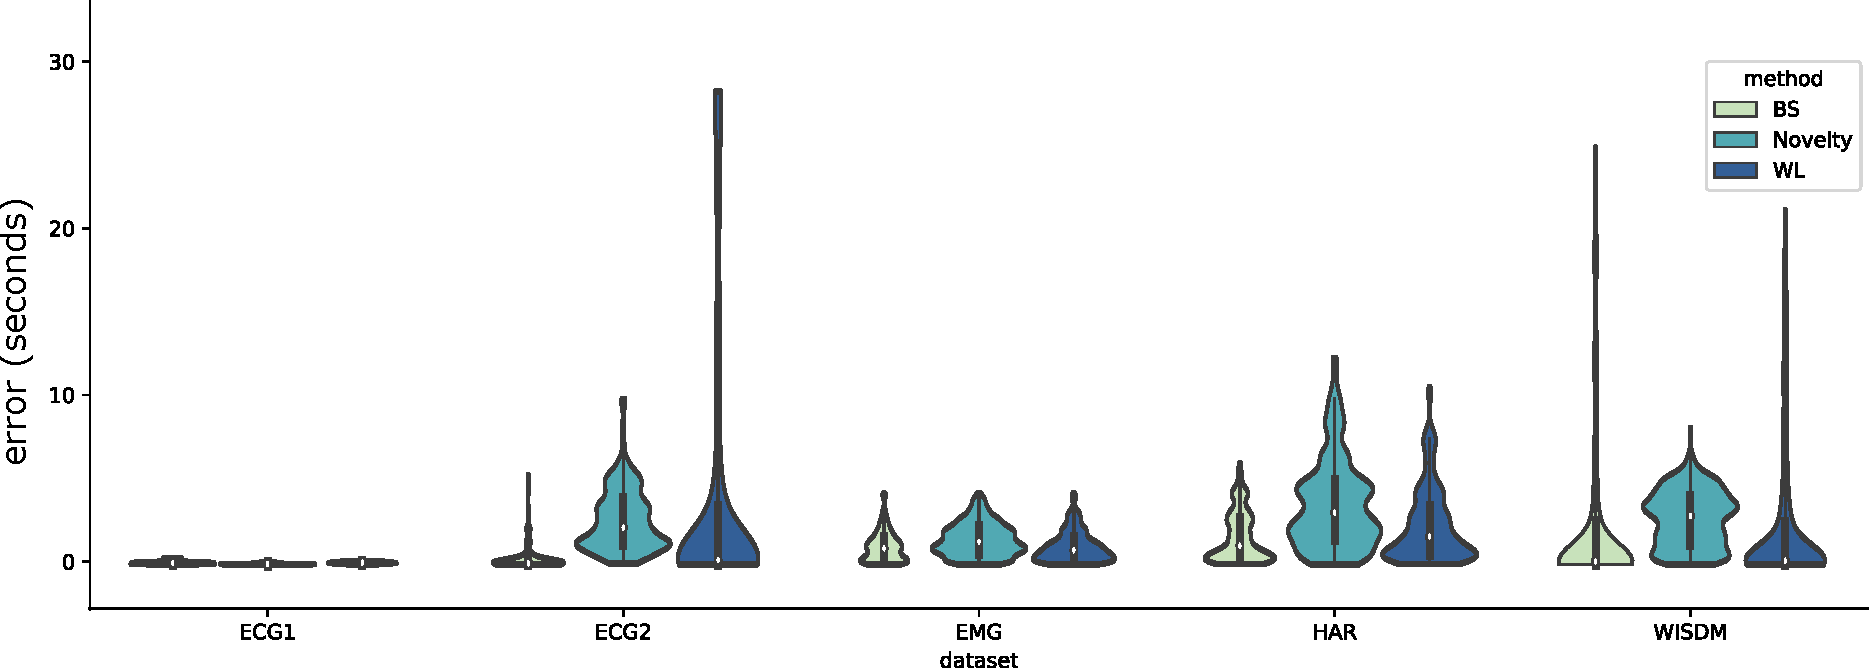
\includegraphics[width=\textwidth]{SSM_distances_summary.pdf}
\caption{Distance values of all $TP$ identified by each method for all datasets. The X-axis indicates the dataset, while the Y-axis indicates the error in seconds as the ratio between the distance in samples and the sampling frequency.}
\label{fig:error_distribution}
\end{figure}

We believe there are several factors that influence the error or precision at which a method can find the changes accurately. These include the sampling frequency of the signal, the timescale at which the events are searched and happen, the labelling errors, and the dimension of the signal. 

A higher sampling frequency with a low timescale segmentation search makes the process less erroneous. In case the task is made on a very large signal (which is the case for \textit{ECG2} signals), low sampling frequency and are searching in a very large timescale (several minutes), than the errors are prone to be much higher. This is the case for datasets \textit{ECG2} and \textit{WISDM}, where higher errors can be accounted by the larger search scale (several minutes in both cases) and large signals with low sampling frequency (20 Hz in case of \textit{WISDM}). We believe this error is reasonable in case the user is exploring the data, but not in cases the user needs very accurate segmentations. 

 \begin{figure}
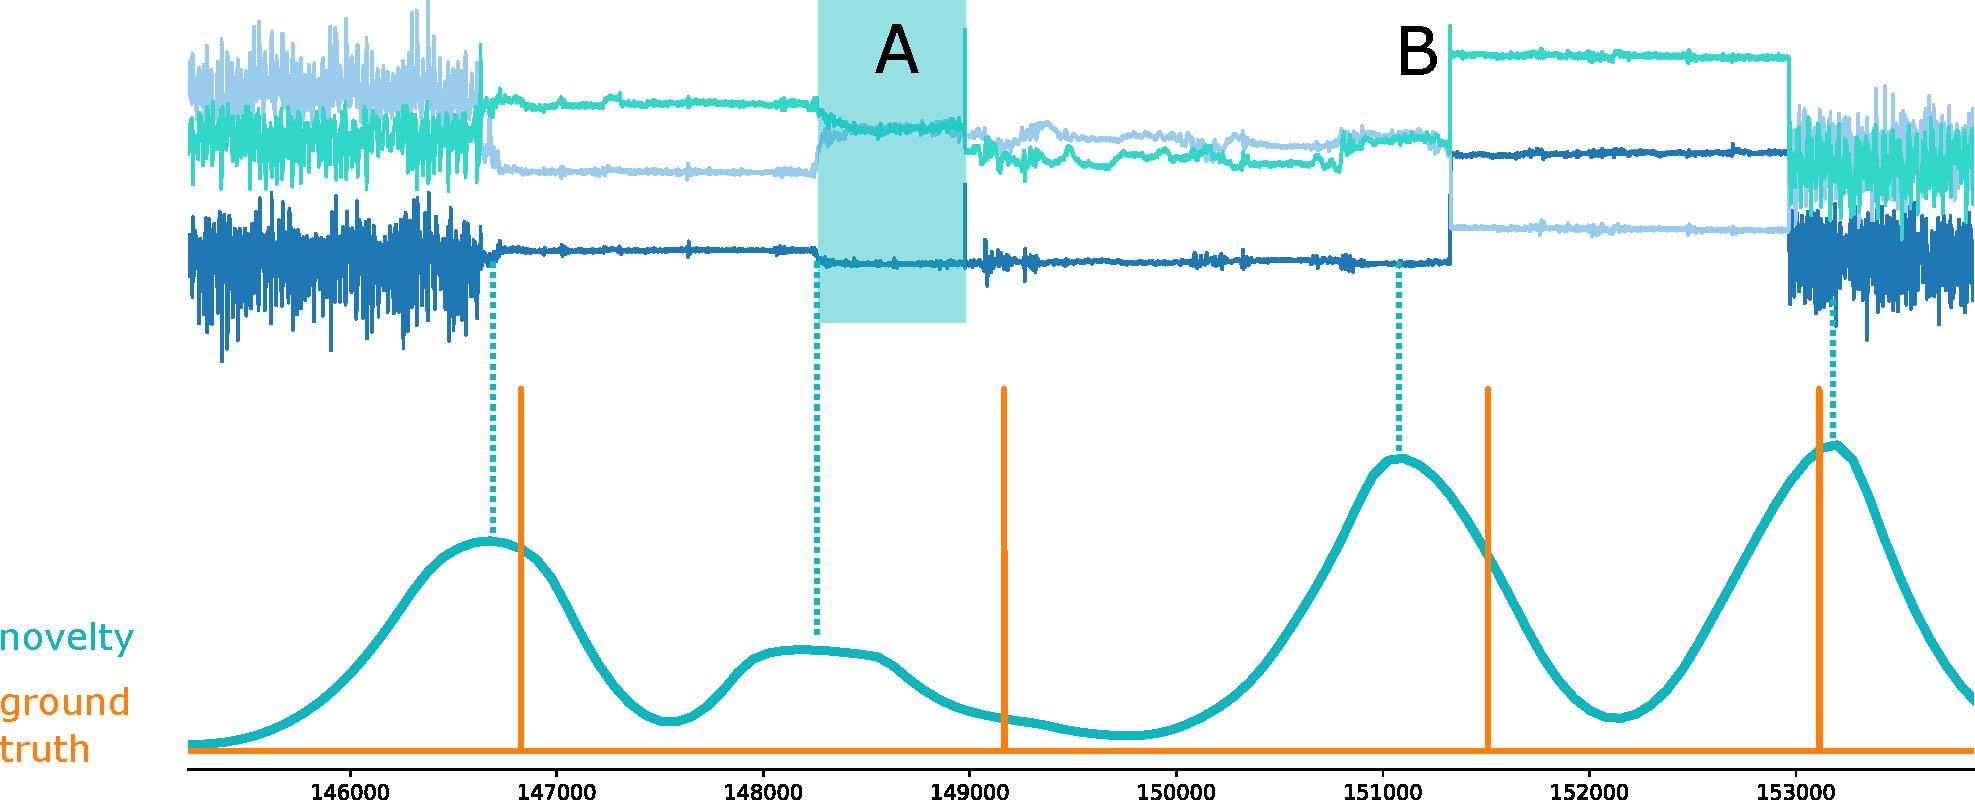
\includegraphics[width=\textwidth]{SSM_explaining_high_distances.pdf}
\caption{Examples of imprecise labelling from Dataset \textit{HAR1}. The 3-axis of the \gls{acc} signal are presented as well as the ground-truth (in orange) and the novelty function (in light blue), computed with the parameters used for the results obtained. Area \textbf{A} indicates the transition from standing to laying, while the transition \textbf{B} indicates the transition from laying to sitting.}
\label{fig:example_badlabel}
\end{figure}

In case of \textit{HAR1}, the increased error can also be explained by the lack of precision in some ground truth labels. As we show in Figure \ref{fig:example_badlabel}, there are ground-truths that do not match precisely where the change happens and this has an effect on the distances. An example is the peak that identifies the transition between sitting and standing (noted as \textbf{B} in Figure \ref{fig:example_badlabel}). In this case, the distance was very high (approximately 500 samples, which accounts for 10 seconds), also because the ground-truth was far from the actual segmentation point. We believe it would be unfair to not count it as a \textit{TP}, but we have to understand the limitations of such imprecise measurement. In addition, another example of imprecise labelling is presented in the same Figure (noted as A), where the change between standing and laying is not sharp and the transition takes some time. The proposed method identifies this change at the beginning of the transition, but the label is made at the end. This was counted as a $FP$, which is unfair. Still, we have to take these limitations into account and reason about how to improve both the method, but also, how to be fair in the evaluation of such segmentation tasks.

Typically, both $WL$ and $BS$ have better results in this aspect, but are not as robust in identifying all segmentation changes, which gives value to the proposed method, but these distance limitations have to be considered. 

\textit{How can we improve the method in being more precise?} The method can be improved if a higher overlap is used. However this also implies that certain conditions are met, namely that the record is not too large, since the matrix might not be able to be entirely computed. Larger records require larger search windows, lower overlap and larger kernel sizes, which reduce the ability to detect short timescale events and make it less precise. One way to counteract this effect is to not compute the entire matrix, but rather only follow its diagonal while sliding the window and extracting the features. In this case, the method could be used with total overlap and the novelty function could be computed with higher precision. In addition, we also believe the detection strategy (using a peak finder) can make it less accurate, since we need a very smooth novelty function for this purpose. One possible strategy could involve the search of higher peaks inside the sliding window, removing all other peaks that could be counted as $FP$.

\section{Novelty Segmentation of Occupational Data}
\label{append:novelty_occupational}

The novelty segmentation and periodic segmentation was performed on the occupational dataset recorded at \textit{Volkswagen Autoeuropa}. The presented results show in Table \ref{tab:auto_scores} the detection of changes that correspond to active to non-active working periods as well as transitions between two different workstations. All these events were annotated manually with the support of the videos available. 

\begin{table}
\caption{Results of type event 1 (work period transition), discriminated per time serie samples. Measurements of \gls{P}, \gls{R}, \gls{F1} of each according sample from Dataset 14 (see Section \ref{dat:dataset_industry}). Signals without changes in activity were not considered (N.A).}
\label{tab:auto_scores}
\centering
\begin{tabular}{lccc}
\toprule
Signal         & \gls{P}    & \gls{R} & \gls{F1}\\
\midrule
Operator 1 Workstation 1      & 0,78 & 1 & 0,88\\
Operator 1 Workstation 2      & 1    & 1 & 1\\
Operator 2 Workstation 1\&2 & 0,86 & 1 & 0,92\\
Operator 3 Workstation 1    & 0,80 & 1 & 0,89\\
Operator 3 Workstation 2 & N.A & N.A & N.A\\
Operator 4 Workstation 1    & 1    & 1 & 1\\
Operator 4 Workstation 2 & N.A & N.A & N.A\\
Operator 5 Workstation 1      & 1    & 1 & 1\\
Operator 5 Workstation 2      & 1    & 1 & 1\\
Operator 6 Workstation 1 & N.A & N.A & N.A\\
Operator 6 Workstation 2 & N.A & N.A & N.A\\ 
\hline
Average & 0.92 & 1 & 0.96\\
\bottomrule
\end{tabular}
\end{table}

\begin{figure}
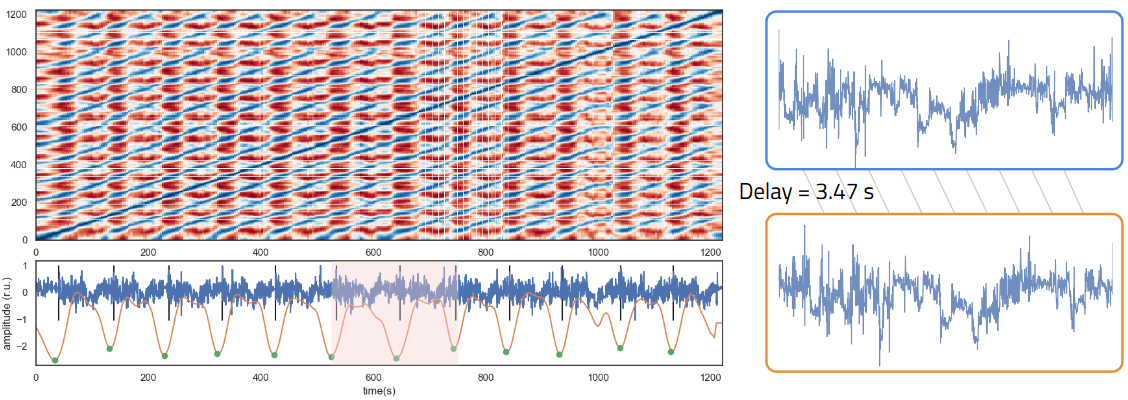
\includegraphics[width=\linewidth]{operator5_red_station_result2.png}
\caption{Example of the detection of working cycles by means of the \gls{ssm} after removing the non-active working periods. Black bars represent the ground truth events, green circles are the detected cycles on the similarity function (orange), represented on the bottom subplot. The X-accelerometer signal from the hand sensor is in blue.}
\label{fig:example_workcycle}
\end{figure}

In Table \ref{tab:wc_results}, the detection of each working period was made with the similarity function. As exemplified in other datasets, the valleys of this function indicate the presence of a period. The novelty function was used to segment the signal in smaller subsequences. For each of these segments, the number of valleys detected was counted, being indicated how many of the working cycles were detected in comparison with the real number of cycles. The criteria for this evaluation are the following:

\begin{enumerate}

\item \textbf{correct detection of cycles}. A cycle segment is considered correct if the moments at which the cycles are segmented correspond to a consistent position on the signal. Even if the segmentation of cycles occurs delayed from the ground-truth selection, what is evaluated in this category is the consistency of the algorithm in defining the working cycle. Here are measured how many cycles are correctly segmented;

\item \textbf{calculate the error between the ground-truth segmentation and the algorithm's segmentation}. The ground-truth duration of cycles is compared with the duration of the detected cycles by calculating the absolute difference between durations. This error is expressed in terms of seconds per cycle and duration percentage of the cycle. Figure \ref{fig:example_workcycle} shows an example of the detection performed, being the duration error how many seconds the interval between dark bars and green circles highlighted on the Figure differ. The percentage indicates the ratio of the working cycle that the duration error corresponds to. 

\end{enumerate}

\begin{table}
\centering
\caption{Detected cycles results of the detection of cycling events, on Dataset 14 (see Section \ref{dat:dataset_industry}).}
\label{tab:wc_results}
\begin{tabular}{lcc} 
\toprule
Signal & Detected Cycles & Duration Error\\ 
\midrule
Operator 1 Workstation 1 & 11/11 & 3.26s (3.04\%)\\
Operator 1 Workstation 2 & 14/15 & 8.09s (7.55\%)\\
Operator 2 Workstation 1 & 14/14 & 6.45s (6.40\%)\\
Operator 2 Workstation 2 & 11/11 & 11.2s (11.39\%)\\
Operator 3 Workstation 1 & 16/16 & 12.35s (11.79\%)\\
Operator 3 Workstation 2 & 13/13 & 11.41s (10.68\%)\\
Operator 4 Workstation 1 & 14/14 & 1.05s (0.4\%)\\
Operator 4 Workstation 2 & 11/11 & 3.42s (3.32\%)\\
Operator 5 Workstation 1 & 12/12 & 2.83s (2.85\%)\\
Operator 5 Workstation 2 & 10/11 & 3.47s (3.45\%)\\
Operator 6 Workstation 1 & 14/15 & 3.79s (3.74\%)\\
Operator 6 Workstation 2 & 14/15 & 5.79s (5.73\%)\\
\midrule
\multicolumn{1}{c}{Total} & 154/157 & N.A.\\
\bottomrule
\end{tabular}
\end{table}

\section{Overall Results of HeaRTS and 1-NN ED on Dataset 1}
\label{app:overall_ucr_results}

\subsection{Additional Results}

In Figure \ref{fig:comparison_with_ed} are displayed the comparison between each text-based method and the 1-NN \gls{ed}. These results show that the methods have a comparable performance with this standard approach. It also shows that the \gls{bow} or \gls{tfidf} models used with an \gls{svm} classifier performed better and tend to have better results. However, additional results should be performed to optimize the intrinsic hyperparameters of both \gls{svm} and \gls{nb} models.

\begin{figure}
\centering
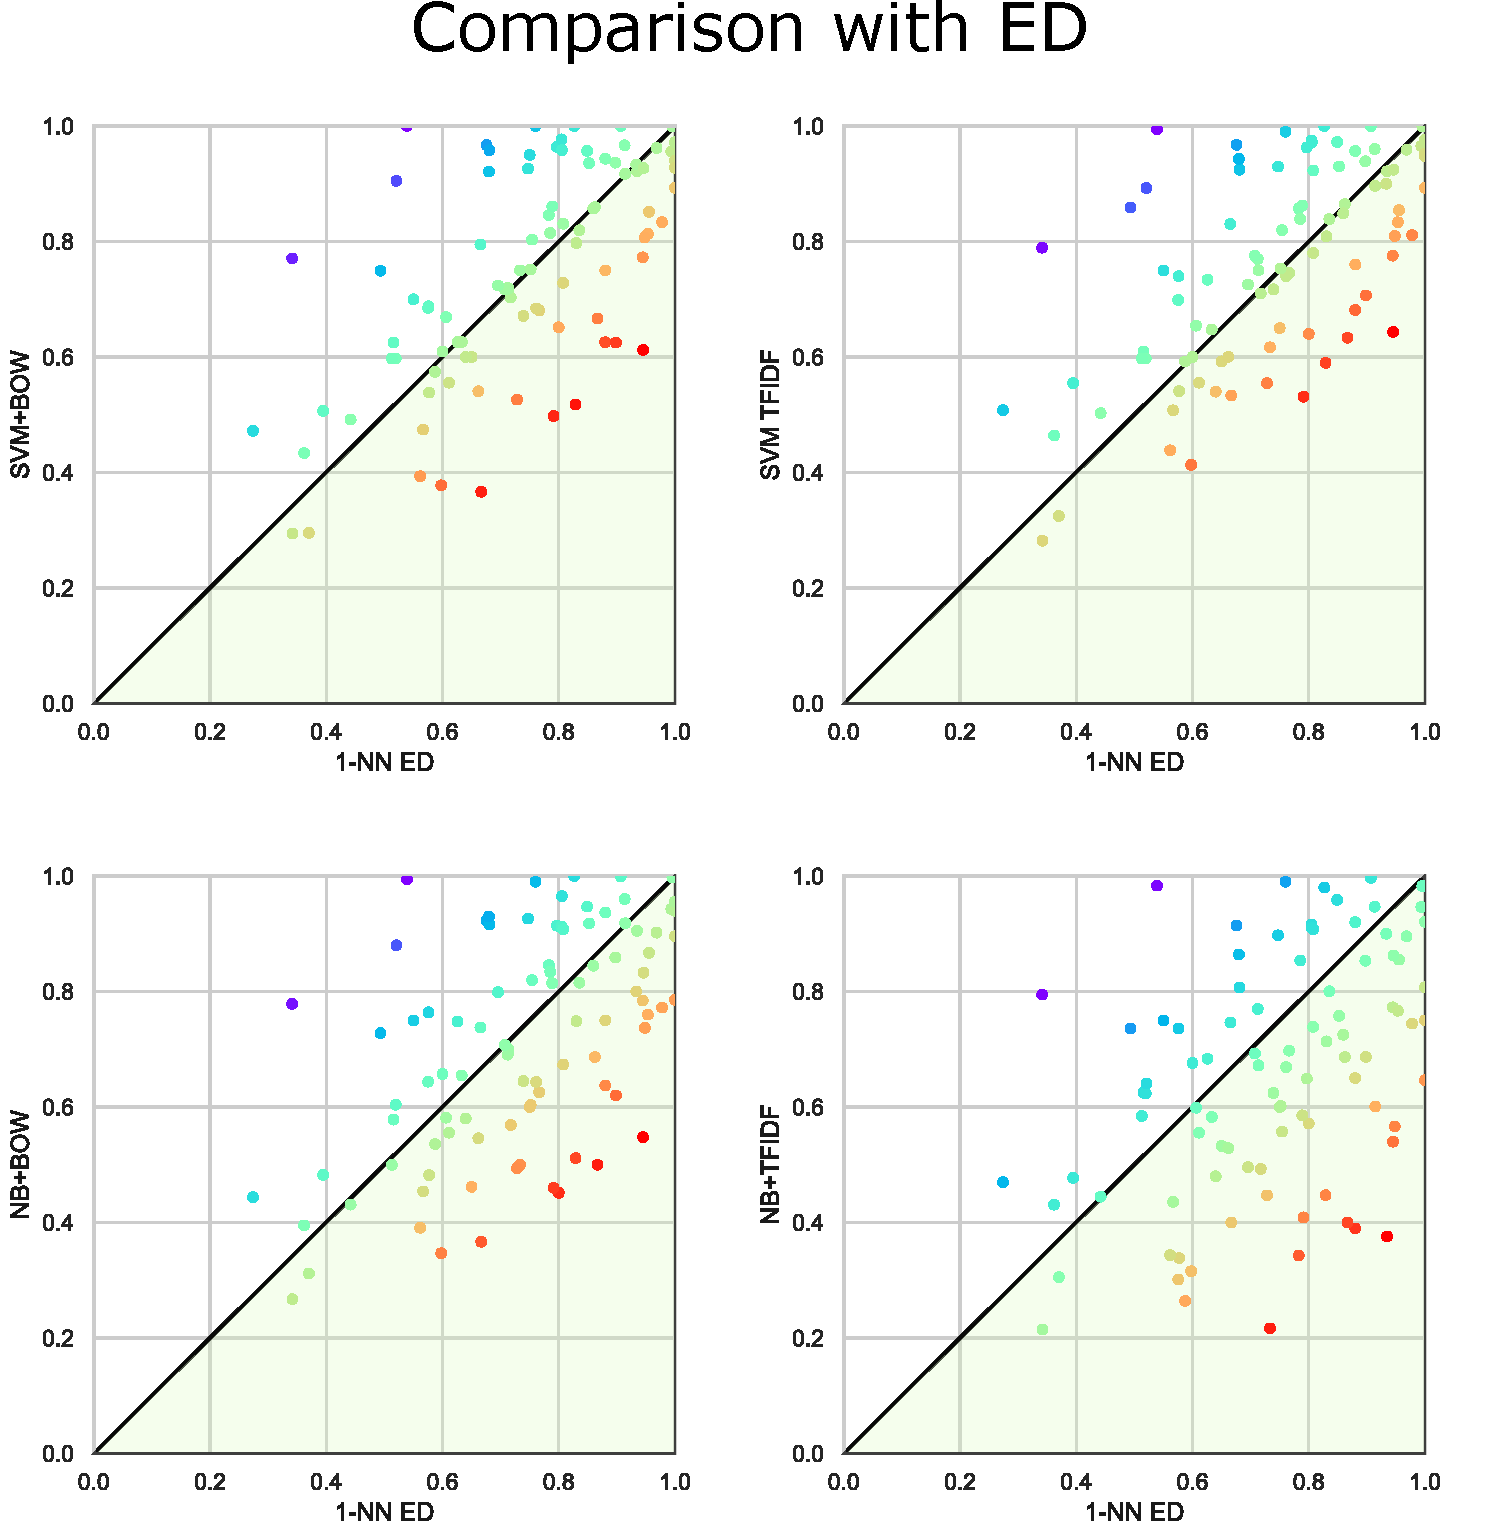
\includegraphics[width=0.75\linewidth]{hearts_comparison_with_ED.pdf}
\caption{Maps with the comparison between each text-based method explored and the 1-NN \gls{ed}.}
\label{fig:comparison_with_ed}
\end{figure}

One relevant difference that was noticed with the usage of the text-based methods (\gls{hearts}), was the decrease in performance when applied on the validation step. Figure \ref{fig:cv_vs_test} shows how this is evident for \gls{hearts}. The performance dropped substantially, suggesting that the text models might not generalize as easily in some cases. The 1-NN \gls{ed} method had a more constant performance.

\begin{figure}
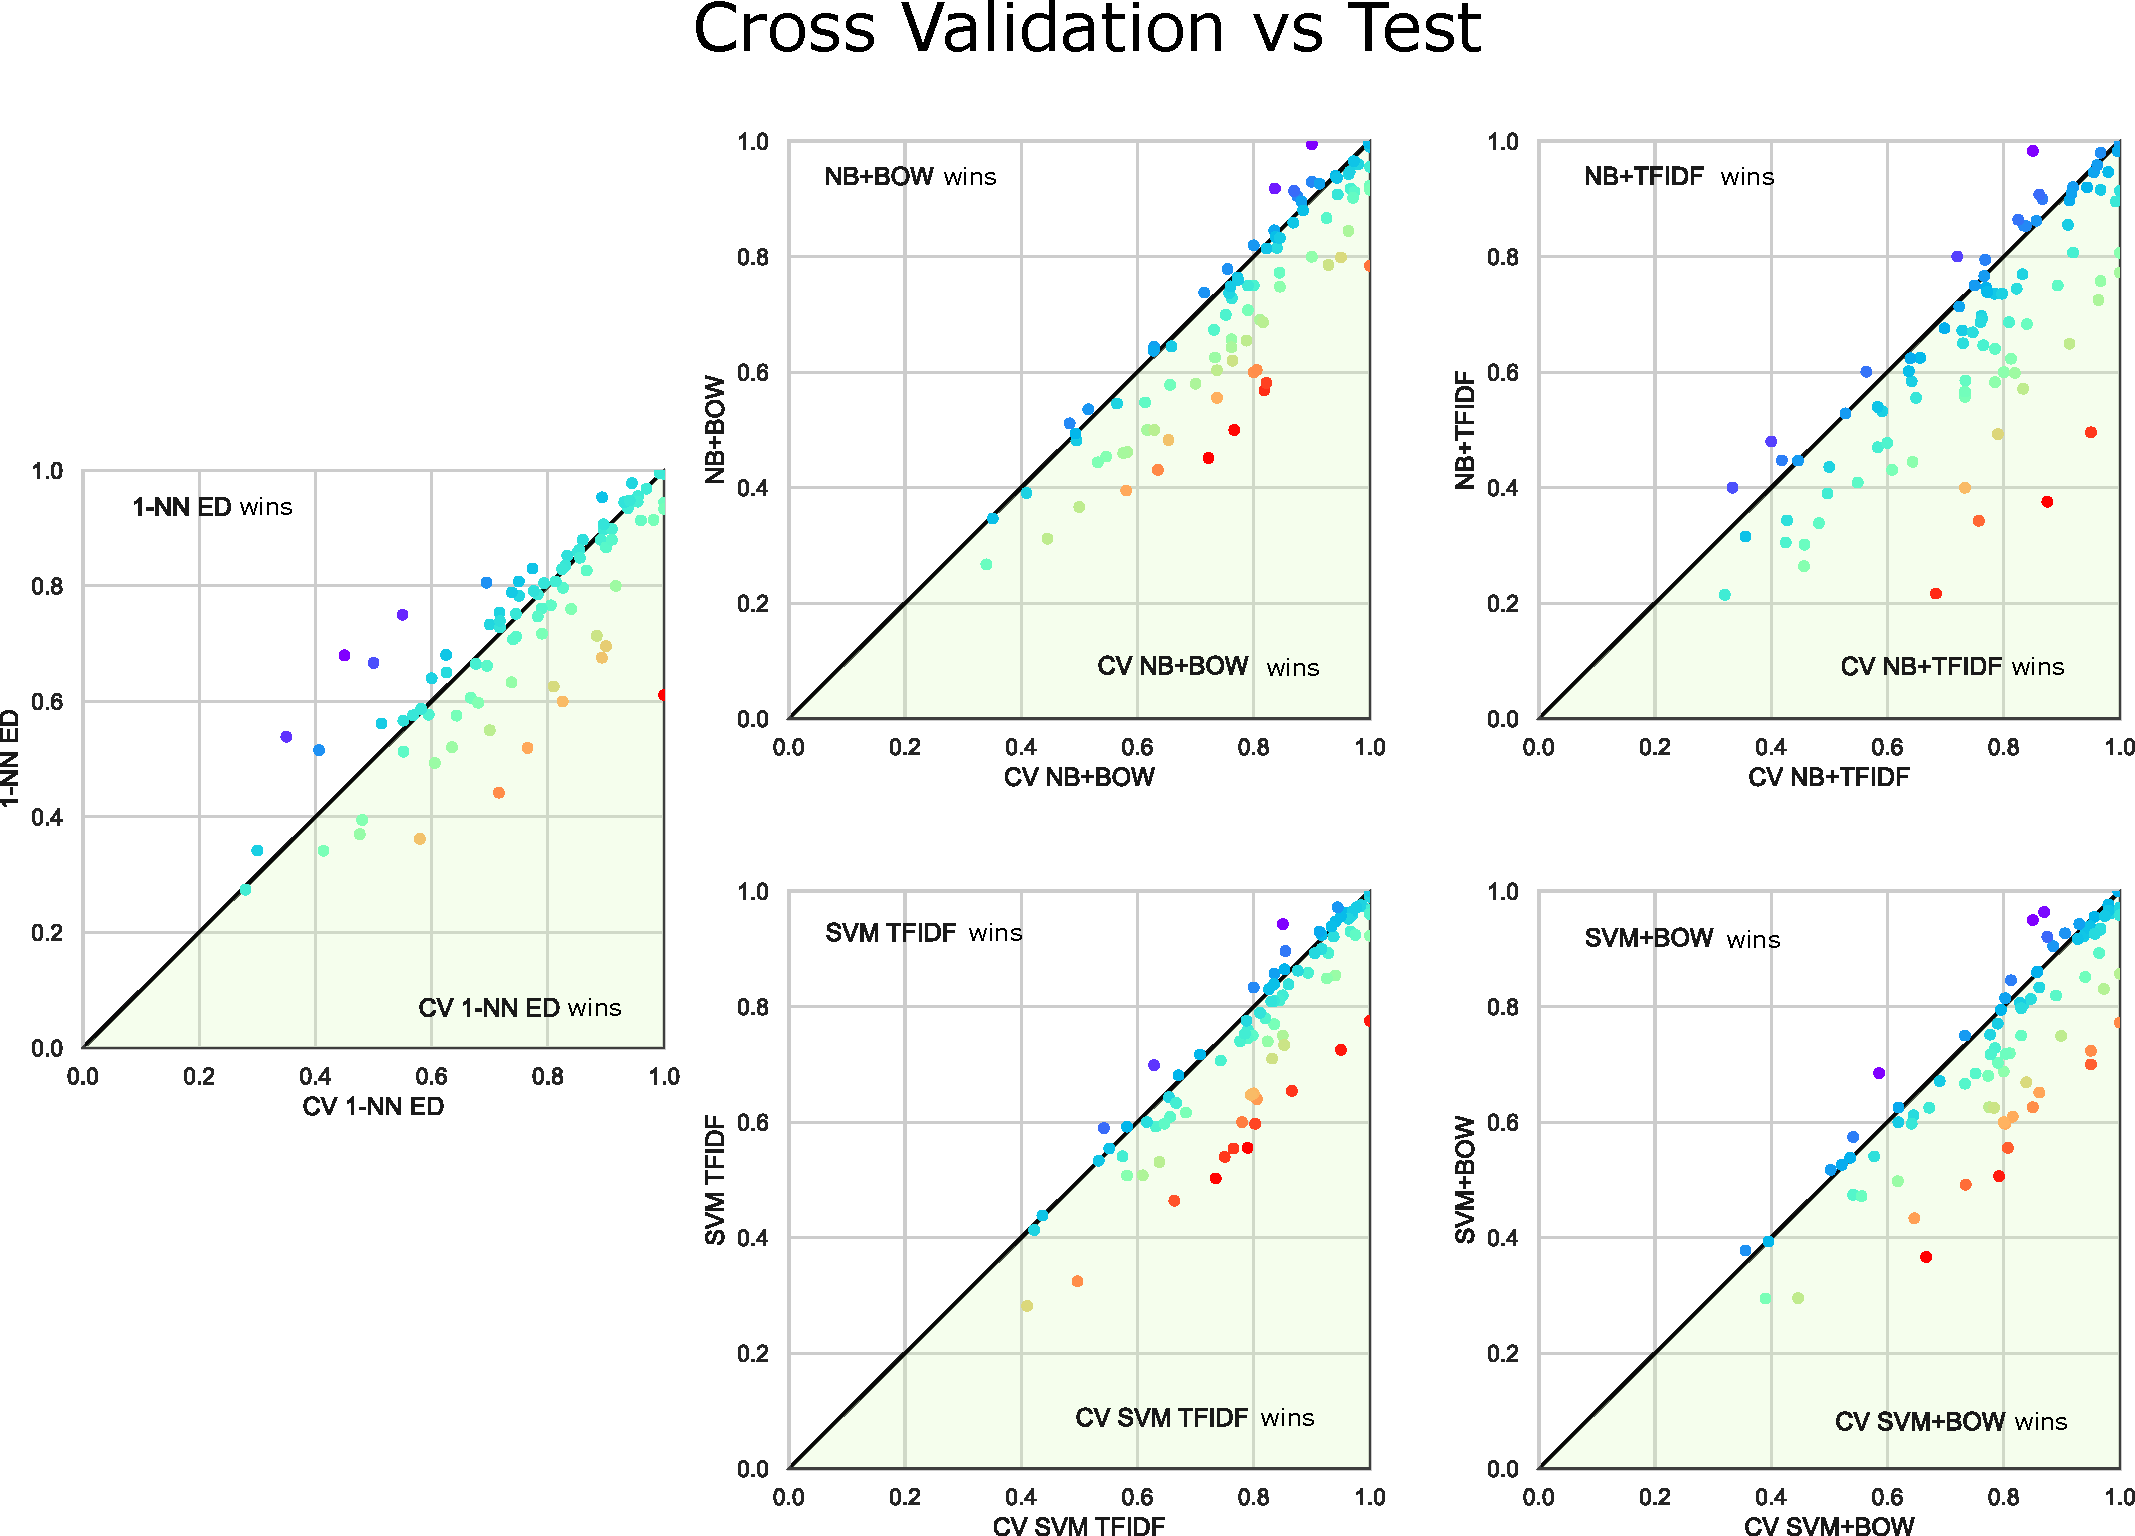
\includegraphics[width=\linewidth]{Hearts_CV_vs_Test.pdf}
\caption{Maps that compare the accuracy of each method during the cross-validation step and test step.}
\label{fig:cv_vs_test}
\end{figure}


\subsection{Accuracies for each dataset}
\label{subsec:hearts_all_accuracies}

In table \ref{tab:ucr_results} are displayed the overall results of all algorithms used on Dataset 1 (\textit{UCRC}, see Section \ref{dat:dat_ucr}). 

\begin{table}
    \centering
    \caption{Overall results when applying \gls{hearts} and 1-NN \gls{ed} on dataset 1. The first column indicates the name of the dataset, and the remaining columns are the name of the algorithms used. V-A: Cross-validation (CV) \gls{bow}+\gls{nb}; A: \gls{bow}+\gls{nb}; V-B: CV \gls{bow}+\gls{svm}; B: \gls{bow}+\gls{svm}; V-C: CV \gls{tfidf}+\gls{nb}; C: \gls{tfidf}+\gls{nb}; V-D: CV \gls{tfidf}+\gls{svm}; D: \gls{tfidf}+{svm}; V-E: CV 1-NN \gls{ed}; E: 1-NN \gls{ed}.}
    \resizebox{\textwidth}{!}{%
    \begin{tabular}{lcccccccccc}
    \toprule
     Dataset & V-A & A & V-B & B & V-C & C & V-D & D & V-E & E \\
     \midrule
        ArrowHead & 0.72 & 0.45 & 0.86 & 0.65 & 0.83 & 0.57 & 0.81 & 0.64 & 0.92 & 0.80 \\ \hline
        Beef & 0.50 & 0.37 & 0.67 & 0.37 & 0.33 & 0.40 & 0.53 & 0.53 & 0.50 & 0.67 \\ \hline
        BeetleFly & 0.80 & 0.60 & 0.85 & 0.95 & 0.80 & 0.60 & 0.80 & 0.65 & 0.55 & 0.75 \\ \hline
        BirdChicken & 0.80 & 0.75 & 0.95 & 0.70 & 0.75 & 0.75 & 0.85 & 0.75 & 0.70 & 0.55 \\ \hline
        BME & 1.00 & 1.00 & 1.00 & 1.00 & 0.97 & 0.98 & 1.00 & 1.00 & 0.87 & 0.83 \\ \hline
        Car & 0.62 & 0.50 & 0.73 & 0.75 & 0.68 & 0.22 & 0.68 & 0.62 & 0.70 & 0.73 \\ \hline
        CBF & 0.97 & 0.92 & 0.97 & 0.94 & 0.97 & 0.76 & 0.97 & 0.93 & 0.83 & 0.85 \\ \hline
        Chinatown & 1.00 & 0.78 & 1.00 & 0.77 & 1.00 & 0.77 & 1.00 & 0.78 & 1.00 & 0.94 \\ \hline
        ChlorineConcentration & 0.58 & 0.46 & 0.62 & 0.60 & 0.59 & 0.53 & 0.63 & 0.59 & 0.63 & 0.65 \\ \hline
        Coffee & 0.93 & 0.79 & 0.96 & 0.89 & 0.89 & 0.75 & 0.93 & 0.89 & 1.00 & 1.00 \\ \hline
        Computers & 0.77 & 0.76 & 0.80 & 0.69 & 0.78 & 0.74 & 0.82 & 0.74 & 0.57 & 0.58 \\ \hline
        CricketX & 0.49 & 0.48 & 0.54 & 0.54 & 0.48 & 0.34 & 0.57 & 0.54 & 0.59 & 0.58 \\ \hline
        CricketY & 0.55 & 0.45 & 0.54 & 0.47 & 0.50 & 0.44 & 0.58 & 0.51 & 0.55 & 0.57 \\ \hline
        CricketZ & 0.52 & 0.54 & 0.54 & 0.57 & 0.46 & 0.26 & 0.58 & 0.59 & 0.58 & 0.59 \\ \hline
        Crop & 0.49 & 0.49 & 0.52 & 0.53 & 0.45 & 0.45 & 0.55 & 0.55 & 0.72 & 0.73 \\ \hline
        DiatomSizeReduction & 0.88 & 0.91 & 0.94 & 0.92 & 0.88 & 0.38 & 0.94 & 0.92 & 0.94 & 0.93 \\ \hline
        DistalPhalanxOutlineAgeGroup & 0.85 & 0.75 & 0.85 & 0.63 & 0.84 & 0.68 & 0.85 & 0.73 & 0.81 & 0.63 \\ \hline
        DistalPhalanxOutlineCorrect & 0.82 & 0.57 & 0.79 & 0.70 & 0.79 & 0.49 & 0.83 & 0.71 & 0.79 & 0.72 \\ \hline
        DistalPhalanxTW & 0.79 & 0.65 & 0.78 & 0.63 & 0.79 & 0.58 & 0.80 & 0.65 & 0.74 & 0.63 \\ \hline
        Earthquakes & 0.81 & 0.69 & 0.81 & 0.72 & 0.83 & 0.77 & 0.84 & 0.77 & 0.75 & 0.71 \\ \hline
        ECG200 & 0.79 & 0.75 & 0.83 & 0.75 & 0.73 & 0.65 & 0.79 & 0.76 & 0.86 & 0.88 \\ \hline
        ECGFiveDays & 0.87 & 0.91 & 0.87 & 0.96 & 0.91 & 0.65 & 0.96 & 0.96 & 0.83 & 0.80 \\ \hline
        EOGHorizontalSignal & 0.64 & 0.43 & 0.73 & 0.49 & 0.64 & 0.44 & 0.73 & 0.50 & 0.72 & 0.44 \\ \hline
        EOGVerticalSignal & 0.58 & 0.40 & 0.65 & 0.43 & 0.61 & 0.43 & 0.66 & 0.46 & 0.58 & 0.36 \\ \hline
        EthanolLevel & 0.53 & 0.44 & 0.56 & 0.47 & 0.58 & 0.47 & 0.61 & 0.51 & 0.28 & 0.27 \\ \hline
        FaceAll & 0.75 & 0.70 & 0.80 & 0.72 & 0.73 & 0.67 & 0.80 & 0.75 & 0.88 & 0.71 \\ \hline
        Fish & 0.84 & 0.85 & 0.81 & 0.85 & 0.76 & 0.34 & 0.84 & 0.86 & 0.75 & 0.78 \\ \hline
        FordA & 0.71 & 0.74 & 0.80 & 0.79 & 0.77 & 0.75 & 0.83 & 0.83 & 0.68 & 0.67 \\ \hline
        FordB & 0.82 & 0.58 & 0.84 & 0.67 & 0.82 & 0.60 & 0.87 & 0.65 & 0.67 & 0.61 \\ \hline
        FreezerRegularTrain & 0.97 & 0.91 & 0.98 & 0.98 & 0.97 & 0.92 & 0.99 & 0.97 & 0.79 & 0.80 \\ \hline
        FreezerSmallTrain & 1.00 & 0.92 & 1.00 & 0.97 & 1.00 & 0.91 & 1.00 & 0.97 & 0.89 & 0.68 \\ \hline
        GunPointAgeSpan & 0.97 & 0.90 & 0.99 & 0.96 & 0.99 & 0.90 & 0.97 & 0.96 & 0.97 & 0.97 \\ \hline
        GunPointMaleVersusFemale & 0.96 & 0.94 & 0.96 & 0.96 & 0.95 & 0.95 & 0.97 & 0.97 & 1.00 & 0.99 \\ \hline
        GunPointOldVersusYoung & 0.94 & 0.94 & 0.95 & 0.94 & 0.92 & 0.92 & 0.96 & 0.95 & 1.00 & 1.00 \\ \hline
        GunPoint & 0.98 & 0.96 & 0.98 & 0.97 & 0.98 & 0.95 & 1.00 & 0.96 & 0.96 & 0.91 \\ \hline
        Ham & 0.76 & 0.66 & 0.82 & 0.61 & 0.70 & 0.68 & 0.78 & 0.60 & 0.83 & 0.60 \\ \hline
        HandOutlines & 0.82 & 0.69 & 0.86 & 0.86 & 0.81 & 0.69 & 0.85 & 0.86 & 0.85 & 0.86 \\ \hline
        Haptics & 0.45 & 0.31 & 0.45 & 0.30 & 0.43 & 0.31 & 0.50 & 0.32 & 0.48 & 0.37 \\ \hline
        Herring & 0.66 & 0.58 & 0.67 & 0.63 & 0.66 & 0.63 & 0.66 & 0.61 & 0.41 & 0.52 \\ \hline
        HouseTwenty & 1.00 & 0.92 & 1.00 & 0.96 & 1.00 & 0.81 & 0.98 & 0.92 & 0.63 & 0.68 \\ \hline
        InlineSkate & 0.34 & 0.27 & 0.39 & 0.29 & 0.32 & 0.21 & 0.41 & 0.28 & 0.30 & 0.34 \\ \hline
        InsectEPGRegularTrain & 1.00 & 0.96 & 1.00 & 0.97 & 0.92 & 0.81 & 0.98 & 0.98 & 1.00 & 1.00 \\ \hline
        InsectEPGSmallTrain & 0.88 & 0.90 & 0.94 & 0.93 & 0.76 & 0.65 & 0.94 & 0.95 & 1.00 & 1.00 \\ \hline
        InsectWingbeatSound & 0.41 & 0.39 & 0.40 & 0.39 & 0.43 & 0.34 & 0.44 & 0.44 & 0.51 & 0.56 \\ \hline
        ItalyPowerDemand & 0.93 & 0.87 & 0.94 & 0.85 & 0.91 & 0.86 & 0.94 & 0.85 & 0.96 & 0.96 \\
        \bottomrule
    \end{tabular}}
    \label{tab:ucr_results}
\end{table}

\begin{table}
    \centering
    \resizebox{\textwidth}{!}{%
    \begin{tabular}{lcccccccccc}
    	\multicolumn{11}{c}{Continues from Table \ref{tab:ucr_results}}\\
    	\toprule
        Dataset & V-A & A & V-B & B & V-C & C & V-D & D & V-E & E \\
        \midrule
        LargeKitchenAppliances & 0.76 & 0.73 & 0.90 & 0.75 & 0.80 & 0.74 & 0.89 & 0.86 & 0.61 & 0.49 \\ \hline
        Lightning2 & 0.80 & 0.82 & 0.83 & 0.80 & 0.73 & 0.56 & 0.85 & 0.82 & 0.72 & 0.75 \\ \hline
        Lightning7 & 0.63 & 0.64 & 0.59 & 0.68 & 0.46 & 0.30 & 0.63 & 0.70 & 0.64 & 0.58 \\ \hline
        Mallat & 0.84 & 0.92 & 0.93 & 0.92 & 0.56 & 0.60 & 0.85 & 0.90 & 0.98 & 0.91 \\ \hline
        Meat & 0.90 & 0.80 & 0.97 & 0.93 & 0.87 & 0.90 & 0.92 & 0.90 & 1.00 & 0.93 \\ \hline
        MelbournePedestrian & 0.61 & 0.55 & 0.64 & 0.61 & 0.58 & 0.54 & 0.65 & 0.64 & 0.93 & 0.95 \\ \hline
        MiddlePhalanxOutlineAgeGroup & 0.81 & 0.60 & 0.80 & 0.60 & 0.81 & 0.62 & 0.80 & 0.60 & 0.77 & 0.52 \\ \hline
        MiddlePhalanxOutlineCorrect & 0.73 & 0.63 & 0.77 & 0.68 & 0.76 & 0.70 & 0.79 & 0.75 & 0.81 & 0.77 \\ \hline
        MiddlePhalanxTW & 0.63 & 0.50 & 0.64 & 0.60 & 0.64 & 0.58 & 0.65 & 0.60 & 0.55 & 0.51 \\ \hline
        MixedShapesSmallTrain & 0.84 & 0.82 & 0.89 & 0.82 & 0.72 & 0.80 & 0.86 & 0.84 & 0.83 & 0.84 \\ \hline
        MixedShapes & 0.87 & 0.86 & 0.95 & 0.94 & 0.84 & 0.85 & 0.93 & 0.94 & 0.90 & 0.90 \\ \hline
        NonInvasiveFetalECGThorax1 & 0.48 & 0.51 & 0.50 & 0.52 & 0.42 & 0.45 & 0.54 & 0.59 & 0.82 & 0.83 \\ \hline
        NonInvasiveFetalECGThorax2 & 0.63 & 0.64 & 0.62 & 0.63 & 0.50 & 0.39 & 0.67 & 0.68 & 0.89 & 0.88 \\ \hline
        OliveOil & 0.77 & 0.50 & 0.73 & 0.67 & 0.73 & 0.40 & 0.67 & 0.63 & 0.90 & 0.87 \\ \hline
        OSULeaf & 0.89 & 0.88 & 0.89 & 0.90 & 0.79 & 0.64 & 0.91 & 0.89 & 0.64 & 0.52 \\ \hline
        PhalangesOutlinesCorrect & 0.76 & 0.64 & 0.75 & 0.68 & 0.75 & 0.67 & 0.78 & 0.74 & 0.79 & 0.76 \\ \hline
        PowerCons & 0.84 & 0.77 & 0.86 & 0.83 & 0.82 & 0.74 & 0.84 & 0.81 & 0.94 & 0.98 \\ \hline
        ProximalPhalanxOutlineAgeGroup & 0.84 & 0.83 & 0.80 & 0.81 & 0.84 & 0.85 & 0.84 & 0.84 & 0.78 & 0.79 \\ \hline
        ProximalPhalanxOutlineCorrect & 0.73 & 0.67 & 0.79 & 0.73 & 0.77 & 0.74 & 0.82 & 0.78 & 0.81 & 0.81 \\ \hline
        ProximalPhalanxTW & 0.79 & 0.71 & 0.78 & 0.72 & 0.76 & 0.69 & 0.79 & 0.78 & 0.74 & 0.71 \\ \hline
        RefrigerationDevices & 0.65 & 0.48 & 0.79 & 0.51 & 0.60 & 0.48 & 0.77 & 0.55 & 0.48 & 0.39 \\ \hline
        Rock & 0.70 & 0.58 & 0.80 & 0.60 & 0.40 & 0.48 & 0.75 & 0.54 & 0.60 & 0.64 \\ \hline
        SemgHandGenderCh2 & 0.76 & 0.62 & 0.78 & 0.63 & 0.76 & 0.69 & 0.74 & 0.71 & 0.91 & 0.90 \\ \hline
        SemgHandMovementCh2 & 0.35 & 0.35 & 0.36 & 0.38 & 0.36 & 0.32 & 0.42 & 0.41 & 0.68 & 0.60 \\ \hline
        SemgHandSubjectCh2 & 0.58 & 0.46 & 0.62 & 0.50 & 0.55 & 0.41 & 0.64 & 0.53 & 0.78 & 0.79 \\ \hline
        ShapeletSim & 0.90 & 0.99 & 1.00 & 1.00 & 0.85 & 0.98 & 1.00 & 0.99 & 0.35 & 0.54 \\ \hline
        ShapesAll & 0.74 & 0.60 & 0.78 & 0.75 & 0.64 & 0.60 & 0.79 & 0.75 & 0.75 & 0.75 \\ \hline
        SmallKitchenAppliances & 0.75 & 0.78 & 0.79 & 0.77 & 0.77 & 0.79 & 0.81 & 0.79 & 0.41 & 0.34 \\ \hline
        SmoothSubspace & 0.77 & 0.76 & 0.85 & 0.81 & 0.77 & 0.77 & 0.80 & 0.83 & 0.89 & 0.95 \\ \hline
        SonyAIBORobotSurface1 & 0.95 & 0.80 & 0.95 & 0.72 & 0.95 & 0.50 & 0.95 & 0.73 & 0.90 & 0.70 \\ \hline
        SonyAIBORobotSurface2 & 0.96 & 0.84 & 1.00 & 0.86 & 0.96 & 0.73 & 0.93 & 0.85 & 0.85 & 0.86 \\ \hline
        StarlightCurves & 0.97 & 0.95 & 0.97 & 0.96 & 0.96 & 0.96 & 0.98 & 0.97 & 0.86 & 0.85 \\ \hline
        Strawberry & 0.84 & 0.83 & 0.91 & 0.93 & 0.86 & 0.86 & 0.92 & 0.92 & 0.95 & 0.95 \\ \hline
        SwedishLeaf & 0.82 & 0.81 & 0.86 & 0.86 & 0.73 & 0.59 & 0.88 & 0.86 & 0.74 & 0.79 \\ \hline
        SyntheticControl & 0.94 & 0.94 & 0.93 & 0.94 & 0.94 & 0.92 & 0.95 & 0.96 & 0.91 & 0.88 \\ \hline
        ToeSegmentation1 & 0.90 & 0.93 & 0.88 & 0.92 & 0.83 & 0.86 & 0.85 & 0.94 & 0.45 & 0.68 \\ \hline
        ToeSegmentation2 & 0.94 & 0.91 & 0.97 & 0.83 & 0.86 & 0.91 & 1.00 & 0.92 & 0.75 & 0.81 \\ \hline
        Trace & 1.00 & 0.99 & 1.00 & 1.00 & 1.00 & 0.99 & 1.00 & 0.99 & 0.84 & 0.76 \\ \hline
        TwoLeadECG & 0.91 & 0.93 & 0.96 & 0.93 & 0.91 & 0.90 & 0.91 & 0.93 & 0.78 & 0.75 \\ \hline
        TwoPatterns & 1.00 & 1.00 & 1.00 & 1.00 & 1.00 & 1.00 & 1.00 & 1.00 & 0.90 & 0.91 \\ \hline
        UMD & 0.97 & 0.97 & 1.00 & 0.96 & 0.92 & 0.91 & 0.94 & 0.97 & 0.69 & 0.81 \\ \hline
        UWaveGestureLibraryAll & 0.76 & 0.74 & 0.83 & 0.81 & 0.73 & 0.57 & 0.83 & 0.81 & 0.94 & 0.95 \\ \hline
        UWaveGestureLibraryX & 0.66 & 0.64 & 0.69 & 0.67 & 0.64 & 0.62 & 0.71 & 0.72 & 0.72 & 0.74 \\ \hline
        UWaveGestureLibraryY & 0.56 & 0.55 & 0.58 & 0.54 & 0.53 & 0.53 & 0.62 & 0.60 & 0.70 & 0.66 \\ \hline
        Wafer & 1.00 & 1.00 & 1.00 & 1.00 & 1.00 & 0.98 & 1.00 & 1.00 & 0.99 & 1.00 \\ \hline
        Wine & 0.74 & 0.56 & 0.81 & 0.56 & 0.65 & 0.56 & 0.79 & 0.56 & 1.00 & 0.61 \\ \hline
        Yoga & 0.76 & 0.75 & 0.83 & 0.80 & 0.72 & 0.71 & 0.83 & 0.81 & 0.77 & 0.83 \\
        \bottomrule
        Average & 0.78	& 0.71	& 0.81	& 0.75	& 0.75	&0.66 &	0.81 &	0.76 &	0.76 &	0.74\\
        \bottomrule
\end{tabular}}
\end{table}